\documentclass[a4paper,12pt,oneside,openany]{book}

% ============================================================================
% DOCUMENTAÇÃO DO PROJETO DE SOFTWARE - EduHub
% ENGENHARIA DE SOFTWARE II
% UNESP - Faculdade de Ciências - Departamento de Computação
% ============================================================================

\usepackage[T1]{fontenc}
\usepackage[utf8]{inputenc}
\usepackage[brazilian]{babel}
\usepackage{indentfirst}
\usepackage{graphicx}
\usepackage{booktabs}
\usepackage{tabularx}
\usepackage{xltabular} % tabelas com colunas X que quebram entre páginas (apêndice)
\usepackage{array}
\usepackage{enumitem}
\usepackage{hyperref}
\usepackage{natbib}
\usepackage{fancyhdr}
\usepackage[section]{placeins}
\usepackage{float}
\usepackage{listings} % blocos de código (padrões de projeto, §3.4)
\lstset{
  language=Java,
  basicstyle=\ttfamily\footnotesize,
  keywordstyle=\bfseries,
  commentstyle=\itshape,
  showstringspaces=false,
  frame=single,
  columns=fullflexible,
  breaklines=true,
  tabsize=2,
  xleftmargin=1em,
}
\usepackage[top=2cm,bottom=2cm,left=2cm,right=2cm]{geometry}

\hypersetup{
    hidelinks,
    pdftitle={Documentação do Projeto de Software - EduHub},
    pdfauthor={Equipe EduHub}
}

\urlstyle{same}

% ----------------------------------------------------------------------------
% Exibição das orientações do template (desligada para a versão final)
% ----------------------------------------------------------------------------
\newif\iforientacoes
\orientacoesfalse

\newcommand{\orientacao}[1]{%
    \iforientacoes
        \begin{quote}
        \small\itshape\textbf{Orientação:} #1
        \end{quote}
    \fi
}

% ----------------------------------------------------------------------------
% Cabeçalho e rodapé
% ----------------------------------------------------------------------------
\renewcommand{\headrulewidth}{0pt}
\fancyhf{}

% ----------------------------------------------------------------------------
% Informações do trabalho
% ----------------------------------------------------------------------------
\newcommand{\school}{Universidade Estadual Paulista ``Júlio de Mesquita Filho'' (UNESP)\\
Faculdade de Ciências -- Bauru\\
Departamento de Computação}
\newcommand{\discipline}{Engenharia de Software II}
\newcommand{\projtitle}{EduHub}
\newcommand{\projsubtitle}{Documentação do Projeto de Software}
\newcommand{\semester}{2026}

\graphicspath{{images/}}

% Figura comparativa desktop (larga) ao lado da versão mobile (estreita/alta).
% Larguras calibradas para que as duas fiquem com alturas parecidas.
% #1 = imagem desktop, #2 = imagem mobile, #3 = legenda, #4 = label
\newcommand{\comparativotela}[4]{%
  \begin{figure}[H]
  \centering
  \begin{minipage}[c]{0.70\textwidth}\centering
    \includegraphics[width=\linewidth]{#1}
  \end{minipage}\hfill
  \begin{minipage}[c]{0.24\textwidth}\centering
    \includegraphics[width=\linewidth]{#2}
  \end{minipage}
  \caption{#3}\label{#4}
  \end{figure}%
}

\title{Documentação do Projeto de Software}
\author{Equipe EduHub}

\begin{document}

% ============================================================================
% CAPA
% ============================================================================
\thispagestyle{empty}
\begin{titlepage}
	\centering

	% Logotipo da UNESP no topo da página
	\vspace*{-12mm}
	
\includegraphics[width=75mm]{AV01A.jpg}\\[8mm]

	{\large\textbf{\school}}

	\vfill

	{\huge\textbf{\projtitle}}\\[5mm]
	{\Large\projsubtitle}

	\vfill

	{\Large\textbf{\discipline}}\\[14mm]

	Arthur Alves Ribeiro Gordo -- RA: 241024293\\[2mm]
	Caio César Souza Oliveira -- RA: 241025702\\[2mm]
	Davi Ferreira de Souza -- RA: 241024676\\[2mm]
	Mário Masao Mukai -- RA: 241022321

	\vfill

	{\large Bauru -- SP\\\semester}
\end{titlepage}

\tableofcontents
\thispagestyle{empty}

\clearpage
\pagestyle{fancy}
\cfoot{\thepage}
\setcounter{page}{1}

% ============================================================================
% CAPÍTULOS
% ============================================================================
% ============================================================================
\chapter{Introdução e Objetivos}
% ============================================================================

O EduHub é um sistema de gestão educacional e comunicação, projetado para ser
implantado em instituições de ensino públicas ou privadas. Este capítulo
apresenta o contexto do problema que motiva o desenvolvimento do software, os
limites do escopo do projeto, uma visão resumida dos requisitos levantados e
os objetivos de qualidade que orientam as decisões de projeto descritas nos
capítulos seguintes.

\section{Contexto do software}

\subsection{Propósito}

O propósito do EduHub é estabelecer um canal de comunicação digital e
fornecer ferramentas de informação entre a instituição de ensino e seus
alunos, substituindo processos manuais e descentralizados de gestão
acadêmica por uma plataforma única, segmentada por perfil de usuário.

\subsection{Funções do produto}

O EduHub deve fornecer acesso personalizado e seguro (segmentado por perfil
administrativo, docente e aluno), um módulo de informação do aluno
(desempenho acadêmico, notas, frequência e horários), um módulo de gestão
docente (registro de informações pelo professor) e um módulo de gestão
administrativa (ferramentas para coordenadores e secretários gerenciarem
dados da escola).

\subsection{Perspectiva do produto}

O EduHub é um sistema autônomo e independente: não é componente de um
sistema maior e não requer interfaces operacionais em tempo real com
sistemas externos. Seus dados primários (cadastro inicial de alunos,
professores e turmas) são inseridos e gerenciados pela própria interface
administrativa do sistema. Após a implantação, o EduHub passa a ser a fonte
primária de dados acadêmicos da instituição.

\subsection{Características dos usuários}

O EduHub é utilizado por três grupos distintos de usuários, cada um com
necessidades, nível de acesso e expertise próprios, conforme resumido na
Tabela~\ref{tab:perfis-usuarios}.

\begin{table}[ht]
\centering
\caption{Perfis de usuários do EduHub.}
\label{tab:perfis-usuarios}
\begin{tabularx}{\textwidth}{p{0.22\textwidth} p{0.10\textwidth} p{0.24\textwidth} X}
\toprule
\textbf{Tipo de usuário} & \textbf{Nível de acesso} & \textbf{Expertise requerida} & \textbf{Visão geral} \\
\midrule
Administrativo (Coordenadores/Secretários) & Alto & Conhecimento médio de sistemas de gestão & Responsável pela manutenção de cadastros, gestão de turmas, horários e comunicação oficial. \\
Professores (Docentes) & Médio & Foco pedagógico; requer interface intuitiva & Inserção frequente de dados acadêmicos, como registro de frequência e notas de avaliações. \\
Alunos & Baixo & Focado na visualização; alta expectativa de acessibilidade móvel & Consulta de informações acadêmicas, como horários, notas e frequência, e recebimento/envio de mensagens via módulo de comunicação. \\
\bottomrule
\end{tabularx}
\end{table}

\section{Escopo}

O EduHub é organizado em módulos que atendem às necessidades específicas dos
três perfis de usuário. Fazem parte do escopo desta versão inicial:

\begin{itemize}[nosep]
    \item \textbf{Acesso e autenticação}: login por credenciais, recuperação
    de senha, gestão de cargos e permissões associados a cada usuário.
    \item \textbf{Informação do aluno}: consulta de desempenho (notas
    parciais, finais e histórico), acompanhamento de frequência e consulta
    de horários, disciplinas e calendário acadêmico.
    \item \textbf{Gestão docente}: lançamento e edição de notas, registro de
    frequência e visualização das turmas e alunos vinculados ao professor.
    \item \textbf{Gestão administrativa}: cadastro de escola, turmas e
    disciplinas, vínculo professor--disciplina, configuração de horários e
    calendário acadêmico, gestão de períodos de matrícula, busca avançada de
    cadastros e geração de relatórios operacionais.
    \item \textbf{Comunicação}: envio de avisos pela administração, caixa de
    entrada do aluno e canal bidirecional de mensagens entre aluno e
    administração, com roteamento por tags de assunto.
\end{itemize}

Ficam explicitamente fora do escopo desta versão:

\begin{itemize}[nosep]
    \item \textbf{Gestão financeira}: o EduHub não incluirá, nesta versão,
    funcionalidades de emissão de boletos, controle de inadimplência ou
    qualquer gestão de mensalidades e pagamentos.
    \item \textbf{Escalabilidade para grandes redes}: esta versão inicial
    não terá arquitetura voltada ao suporte de um número grande de usuários;
    recursos de escalabilidade e performance para grandes redes escolares
    ficam fora do escopo.
\end{itemize}

\section{Visão geral dos requisitos}

Os requisitos do EduHub foram organizados em seis grupos funcionais e cinco
categorias de requisitos não funcionais. As Tabelas~\ref{tab:rf-resumo}
e~\ref{tab:rnf-resumo} apresentam uma visão resumida de cada grupo.

\begin{table}[ht]
\centering
\caption{Grupos de requisitos funcionais do EduHub.}
\label{tab:rf-resumo}
\begin{tabularx}{\textwidth}{p{0.28\textwidth} p{0.14\textwidth} X}
\toprule
\textbf{Grupo funcional} & \textbf{RFs} & \textbf{Descrição resumida} \\
\midrule
Acesso e Autenticação & RF-01 a RF-13 & Login, recuperação de senha, histórico de acesso e gestão de cargos, hierarquia e permissões. \\
Gestão e Estrutura & RF-14 a RF-20 & Cadastro da escola, turmas, disciplinas, horários, calendário acadêmico e vínculo professor--disciplina. \\
Gestão Acadêmica & RF-21 a RF-27 & Lançamento e edição de notas, registro de frequência, cálculo automático de faltas e trava de período letivo. \\
Informação e Consulta do Aluno & RF-28 a RF-34 & Consulta a boletim, frequência, grade de horários, calendário e solicitação de documentos. \\
Comunicação e Notificações & RF-35 a RF-41 & Comunicados da administração, notificações por e-mail, caixa de entrada e mensagens com roteamento por tag de assunto. \\
Relatórios e Auditoria & RF-42 a RF-45 & Geração e exportação de relatórios acadêmicos e log de alterações e auditoria. \\
\bottomrule
\end{tabularx}
\end{table}

\begin{table}[ht]
\centering
\caption{Requisitos não funcionais do EduHub.}
\label{tab:rnf-resumo}
\begin{tabularx}{\textwidth}{p{0.12\textwidth} p{0.26\textwidth} X}
\toprule
\textbf{ID} & \textbf{Requisito} & \textbf{Descrição resumida} \\
\midrule
RNF-01 & Tempo de resposta & Operações críticas em menos de 2 segundos. \\
RNF-02 & Capacidade de transação & Até 10.000 transações por minuto em picos. \\
RNF-03 & Criptografia & Dados sensíveis, senhas e e-mails criptografados em repouso. \\
RNF-04 & Autenticação de dois fatores & 2FA opcional para os perfis administrativo e docente. \\
RNF-05 & Disponibilidade & Disponibilidade mínima de 99\% ao ano. \\
RNF-06 & Backup e restauração & Backups diários com restauração completa do sistema. \\
RNF-07 & Modularidade & Arquitetura modular que permite evoluir sem impacto entre módulos. \\
RNF-08 & Portabilidade & Aplicação web responsiva em Chrome, Firefox, Safari, Windows e macOS. \\
RNF-09 & Usabilidade & Interface intuitiva adaptada ao perfil de cada usuário. \\
RNF-10 & Acessibilidade & Conformidade com as diretrizes WCAG 2.1. \\
\bottomrule
\end{tabularx}
\end{table}

A especificação detalhada e completa dos requisitos, que inclui todos os
45 requisitos funcionais, os 10 requisitos não funcionais, as 18 histórias
de usuário e os casos de uso, encontra-se no Apêndice~\ref{apx:requisitos}.

\section{Objetivos de qualidade}\label{sec:quality-goals}

Os objetivos de qualidade do EduHub foram definidos a partir dos atributos
de qualidade de produto da norma ISO/IEC 25010 (Figura~\ref{fig:iso25010}),
selecionando-se apenas os atributos com impacto direto sobre as decisões de
projeto: manutenibilidade, segurança, usabilidade, confiabilidade,
portabilidade e desempenho. Cada atributo está diretamente ligado a um ou
mais requisitos não funcionais levantados na especificação.

\begin{figure}[ht]
\centering
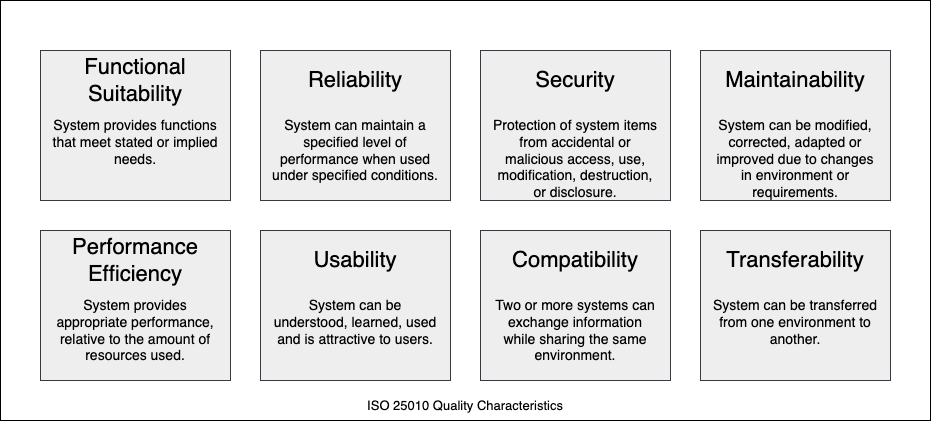
\includegraphics[width=\textwidth]{01_2_iso-25010-topics-EN.drawio.png}
\caption{Características de qualidade de produto da norma ISO/IEC 25010, utilizadas como referência para a seleção dos objetivos de qualidade do EduHub.}
\label{fig:iso25010}
\end{figure}

A manutenibilidade é central para o EduHub por se tratar de um sistema
composto por múltiplos módulos independentes (acesso, gestão acadêmica,
gestão administrativa e comunicação), o que exige arquitetura modular,
alta coesão e baixo acoplamento para permitir a adição de novos recursos
sem impactar os módulos existentes. A segurança é prioritária por lidar com
dados pessoais de alunos e professores sujeitos à LGPD, exigindo
criptografia de credenciais e dados sensíveis e a possibilidade de
autenticação em dois fatores. A usabilidade é fundamental dado o perfil
heterogêneo dos usuários (do administrativo, com maior expertise, ao aluno,
focado em consulta rápida via dispositivos móveis), exigindo interfaces
intuitivas e acessíveis. A confiabilidade garante a continuidade do serviço,
que passa a ser a fonte primária de dados acadêmicos da instituição após a
implantação. A portabilidade assegura o funcionamento correto em diferentes
navegadores e sistemas operacionais, dado que o EduHub é entregue como
aplicação web responsiva. Por fim, o desempenho é relevante em operações
críticas, como autenticação e lançamento de notas em períodos de pico
(por exemplo, fechamento de bimestre).

A Tabela~\ref{tab:objetivos-qualidade} sintetiza esses objetivos, sua
prioridade e o impacto esperado sobre o projeto.

\begin{table}[ht]
\centering
\caption{Objetivos de qualidade do EduHub.}
\label{tab:objetivos-qualidade}
\setlength{\tabcolsep}{10pt}
\begin{tabularx}{\textwidth}{p{0.16\textwidth} p{0.12\textwidth} X}
\toprule
\textbf{Objetivo} & \textbf{Prioridade} & \textbf{Impacto esperado no projeto} \\
\midrule
Manutenibilidade & Alta & Arquitetura modular que permite adicionar recursos sem impactar módulos existentes, exigindo alta coesão e baixo acoplamento no código (RNF-07). \\
Segurança & Alta & Criptografia em repouso de dados cadastrais sensíveis, senhas e e-mails (RNF-03), com suporte opcional a autenticação de dois fatores para perfis administrativo e docente (RNF-04). \\
Desempenho & Alta & Tempo de resposta inferior a 2 segundos em operações críticas (RNF-01) e capacidade de processar até 10.000 transações por minuto em períodos de pico (RNF-02). \\
Usabilidade & Alta & Interface intuitiva, com navegação clara adaptada ao nível de proficiência de cada perfil de usuário (RNF-09), e acessibilidade conforme WCAG 2.1 (RNF-10). \\
Confiabilidade & Média & Disponibilidade mínima de 99\% ao ano (RNF-05) e backups automáticos diários com restauração completa do sistema (RNF-06). \\
Portabilidade & Média & Funcionamento correto como aplicação web responsiva nos principais navegadores (Chrome, Firefox, Safari) e sistemas operacionais (Windows, macOS) (RNF-08). \\
\bottomrule
\end{tabularx}
\end{table}

% ============================================================================
\chapter{Arquitetura do Sistema}
% ============================================================================

Este capítulo apresenta a arquitetura proposta para o EduHub a partir das
restrições, premissas e requisitos não funcionais definidos no Capítulo 1. A
arquitetura é modelada segundo o
padrão C4, com diagramas de contexto (Nível 1), de contêineres (Nível 2) e de
componentes (Nível 3). As decisões descritas derivam diretamente dessas
restrições e requisitos.

\section{Contexto e fronteiras do sistema}

O EduHub é um sistema autônomo e independente,
que não é componente de um sistema maior e não depende de sistemas acadêmicos
legados nem de gateways de pagamento durante a operação. Sua única integração
externa é com um serviço de e-mail, usado para o envio de notificações
(RF-36). Os dados primários do sistema são inseridos e mantidos pela própria
interface administrativa e, após a implantação, o EduHub passa a ser a fonte
primária dos dados acadêmicos da instituição.

A Figura~\ref{fig:c4-contexto} apresenta o diagrama de contexto (C4, Nível
1). A fronteira do sistema compreende o próprio EduHub, os três perfis de
usuário (Administrativo, Professor e Aluno), descritos na
Tabela~\ref{tab:perfis-usuarios}, e o serviço de e-mail externo. A única
outra dependência externa é operacional, a infraestrutura de servidor de
produção fornecida pela equipe de TI da instituição (D-1, ver
Seção~\ref{sec:restricoes-arquitetura}), e não uma integração de dados.

\begin{figure}[ht]
\centering
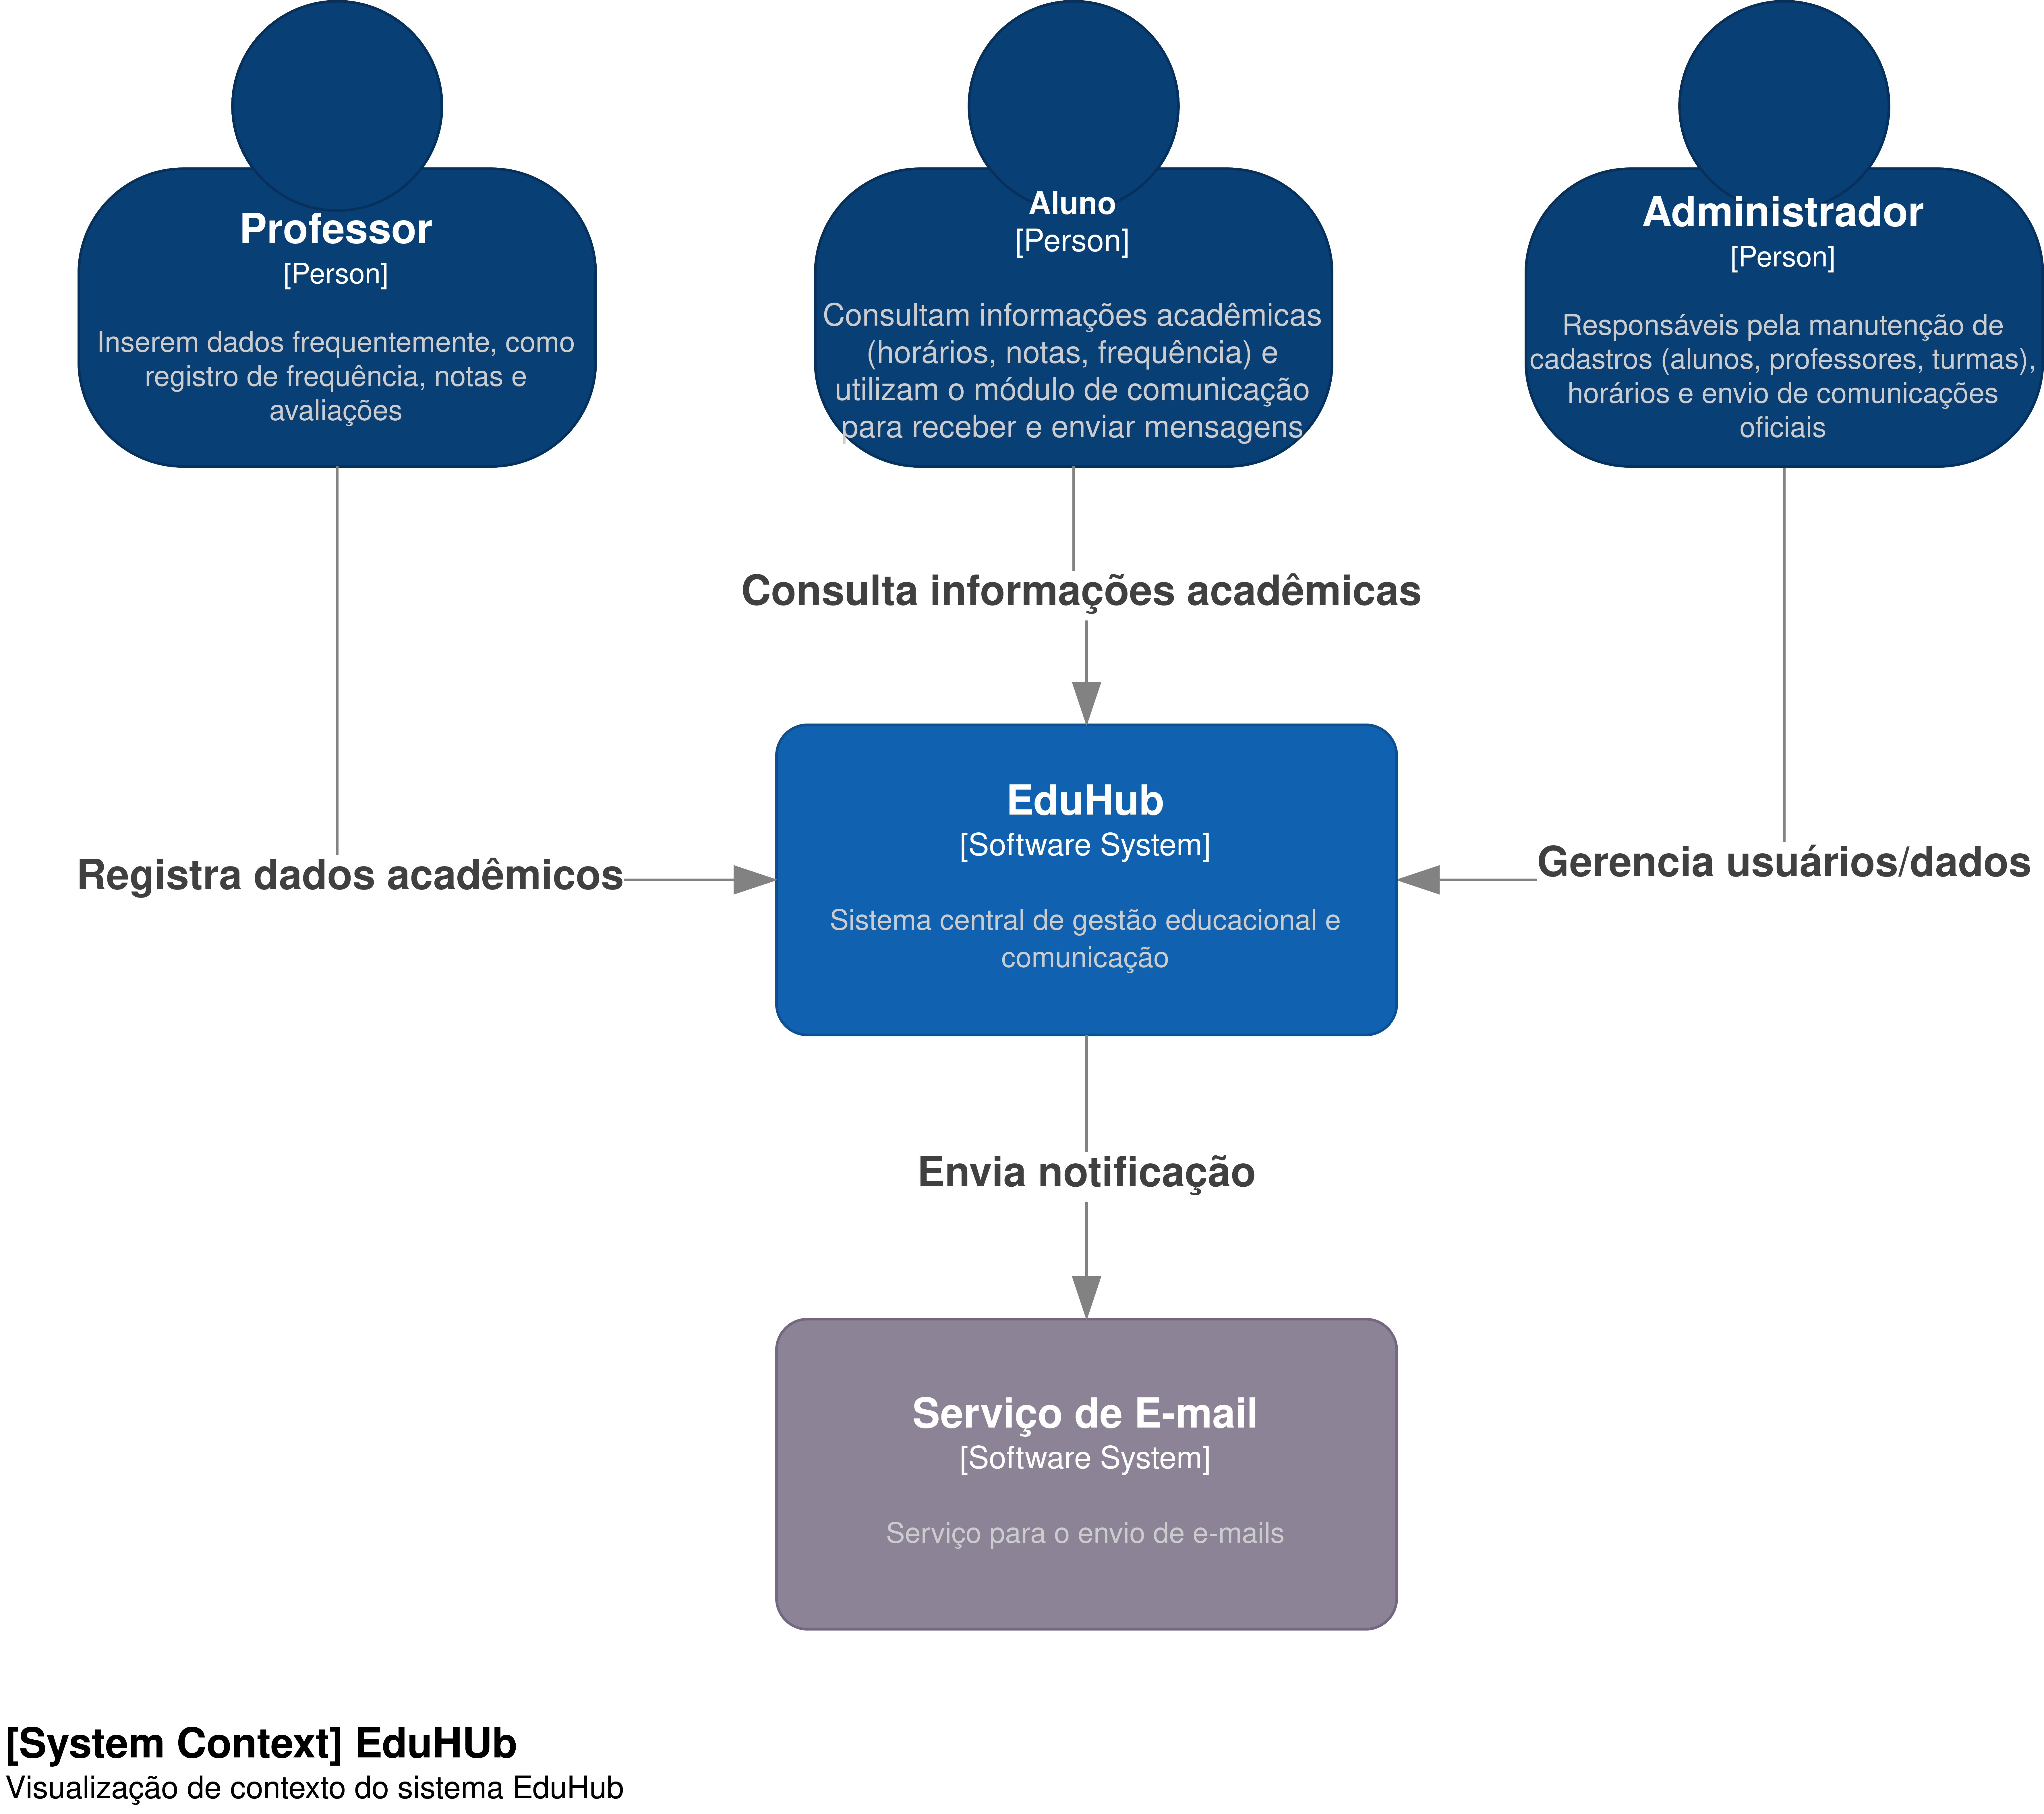
\includegraphics[width=\textwidth]{c4-contexto.png}
\caption{Diagrama de contexto do EduHub (C4 -- Nível 1). Fonte: elaboração própria da equipe.}
\label{fig:c4-contexto}
\end{figure}

\section{Estilo ou padrão arquitetural}

O EduHub adota uma organização modular por domínio funcional, derivada do
RNF-07. O sistema é estruturado em módulos que correspondem às áreas de
funcionalidade identificadas no Capítulo 1: Acesso e Autenticação, Cadastros
e Gestão da Estrutura, Gestão Acadêmica, Informação e Consulta do Aluno,
Comunicação e Notificações, e Relatórios e Auditoria. Cada módulo encapsula
suas próprias regras de negócio e dados, o que reduz o acoplamento entre
áreas que evoluem em ritmos diferentes. Por exemplo, o módulo de Comunicação
pode receber novos recursos sem alterar o módulo de Gestão Acadêmica.

Essa organização modular sustenta o objetivo de qualidade de
manutenibilidade, apontado na Seção~\ref{sec:quality-goals} como prioridade
alta, uma vez que módulos com fronteiras claras favorecem alta coesão e baixo
acoplamento.

\section{Contêineres e componentes}

A arquitetura do EduHub foi modelada seguindo o padrão C4. Os diagramas de
contêineres (Nível 2) e de componentes (Nível 3) detalham a estrutura interna
do sistema a partir da visão de contexto.

No Nível 2 (contêineres), ilustrado na Figura~\ref{fig:c4-container}, o EduHub
é decomposto em três contêineres:
\begin{itemize}[nosep]
    \item \textbf{Frontend}: aplicação web responsiva acessada pelos usuários
    via navegador, que concentra as telas de login, cadastro, grade horária e
    demais interfaces.
    \item \textbf{Backend}: responsável pela lógica de negócio e pela API que
    atende às requisições do Frontend por meio de chamadas JSON/HTTP.
    \item \textbf{Banco de Dados}: armazena os dados de alunos, disciplinas e
    demais informações acadêmicas.
\end{itemize}
O Backend lê e escreve no Banco de Dados e solicita ao serviço de e-mail
externo o envio das notificações.

\begin{figure}[ht]
\centering
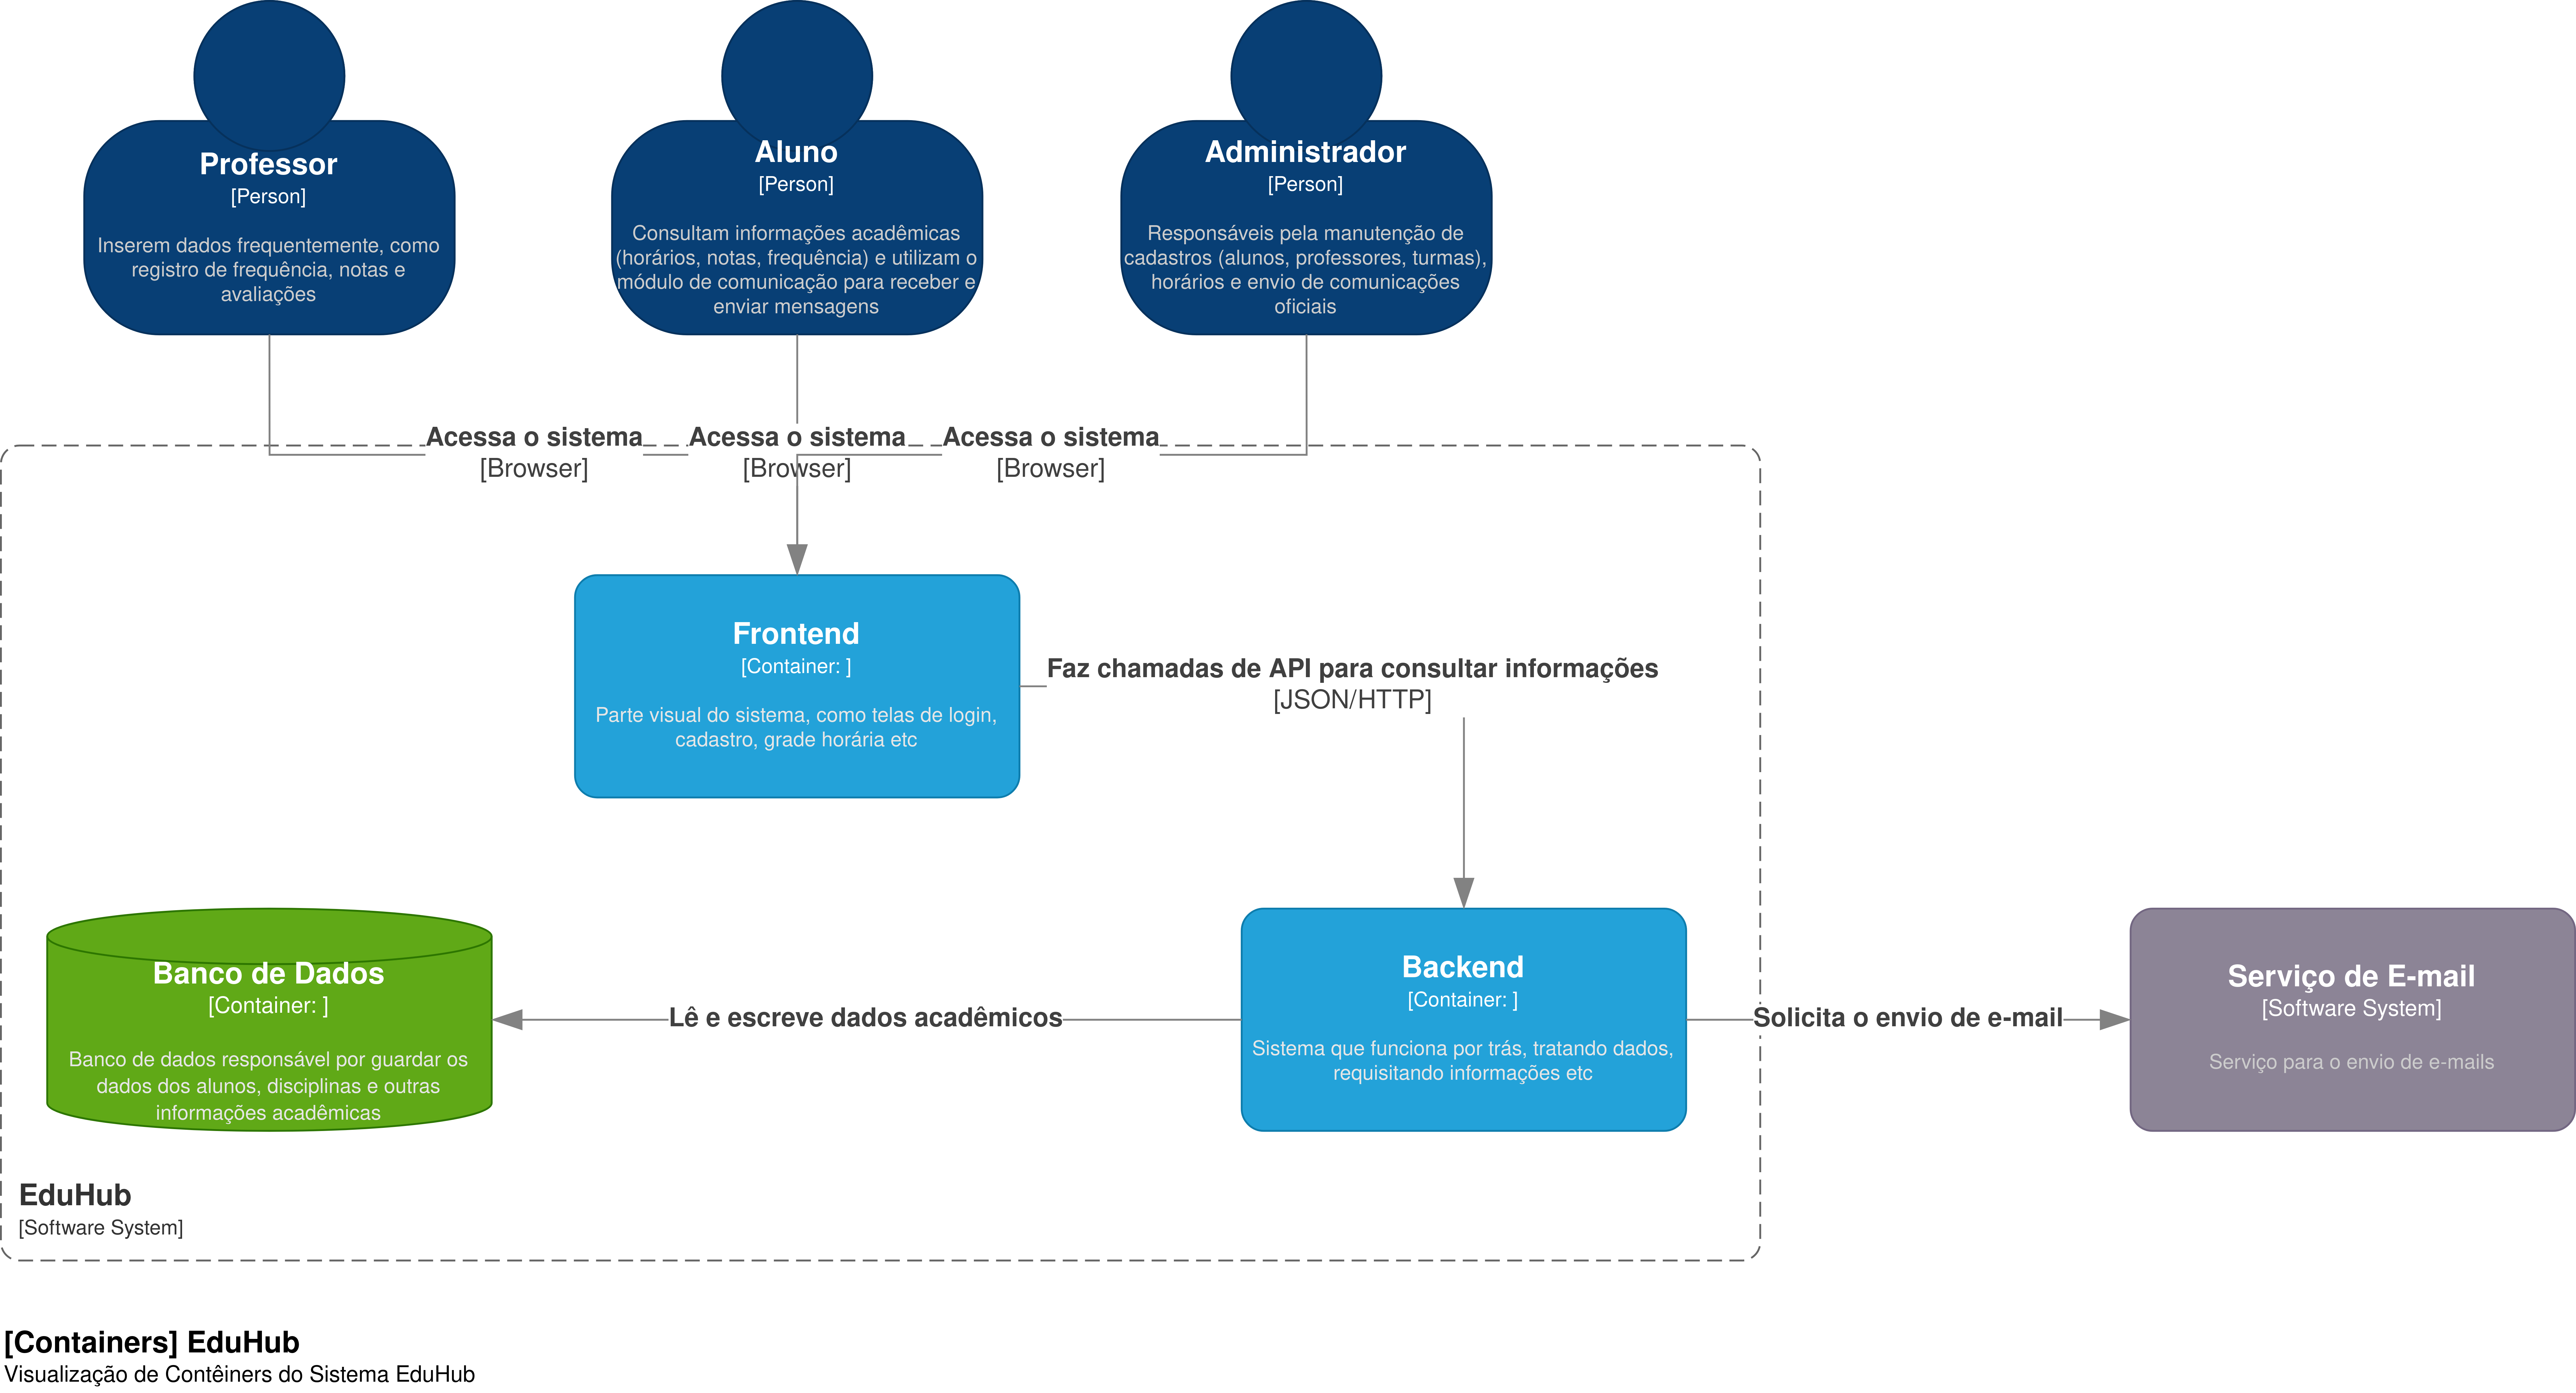
\includegraphics[width=\textwidth]{c4-container.png}
\caption{Diagrama de contêineres do EduHub (C4 -- Nível 2). Fonte: elaboração própria da equipe.}
\label{fig:c4-container}
\end{figure}

Cada contêiner do Backend concentra os módulos funcionais do sistema. A
Tabela~\ref{tab:modulos} consolida esses módulos e suas responsabilidades,
servindo de ponte entre os requisitos e os componentes detalhados a seguir.

\begin{table}[H]
\centering
\caption{Módulos funcionais do EduHub.}
\label{tab:modulos}
\begin{tabularx}{\textwidth}{p{0.28\textwidth} X}
\toprule
\textbf{Módulo} & \textbf{Responsabilidade principal} \\
\midrule
Acesso e Autenticação & Autenticação de usuários por credencial, recuperação
de senha, gestão de cargos, hierarquia e permissões (RF-01 a RF-13). \\
Cadastros e Gestão da Estrutura & Cadastro de dados da escola, turmas,
disciplinas, horários, calendário acadêmico e vínculo professor-disciplina
(RF-14 a RF-20). \\
Gestão Acadêmica & Lançamento e edição de notas, registro de frequência,
cálculo automático de faltas e travamento de períodos letivos (RF-21 a
RF-27). \\
Informação e Consulta do Aluno & Consulta a boletim, frequência, grade de
horários, calendário e solicitação de documentos pelo aluno (RF-28 a
RF-34). \\
Comunicação e Notificações & Envio de comunicados pela administração,
notificações por e-mail, caixa de entrada e mensagens do aluno com roteamento
por tag de assunto (RF-35 a RF-41). \\
Relatórios e Auditoria & Geração e exportação de relatórios acadêmicos e
consulta ao log de alterações e auditoria (RF-42 a RF-45). \\
\bottomrule
\end{tabularx}
\end{table}

No Nível 3 (componentes), ilustrado na Figura~\ref{fig:c4-componentes}, o
contêiner Backend é detalhado em oito componentes que correspondem, em
conjunto, aos módulos funcionais da Tabela~\ref{tab:modulos}:
\begin{itemize}[nosep]
    \item \textbf{Autenticação e Acesso}: login, 2FA e permissões.
    \item \textbf{Gestão de Usuários}: cadastro de alunos, professores e
    administradores.
    \item \textbf{Estrutura Escolar}: cadastro base de escola, turmas e
    disciplinas.
    \item \textbf{Autoatendimento do Aluno}: consulta de boletim, grade
    horária e calendário.
    \item \textbf{Registro Acadêmico}: lançamento de notas e frequência.
    \item \textbf{Mensageria e Comunicação}: caixa de entrada do aluno e
    envio de avisos.
    \item \textbf{Adaptador de E-mail}: formata e dispara os e-mails.
    \item \textbf{Relatório e Auditoria}: geração de relatórios e gravação de
    logs.
\end{itemize}
Os componentes gravam seus dados no Banco de Dados. O Adaptador de E-mail
isola a comunicação com o serviço de e-mail externo, recebendo o e-mail não
formatado da Mensageria, formatando-o e disparando-o para o serviço externo.

\begin{figure}[ht]
\centering
\includegraphics[width=\textwidth]{c4-componentes.png}
\caption{Diagrama de componentes do Backend do EduHub (C4 -- Nível 3). Fonte: elaboração própria da equipe.}
\label{fig:c4-componentes}
\end{figure}


\section{Decisões arquiteturais relevantes}

A tabela a seguir registra as decisões arquiteturais que decorrem
diretamente das restrições e requisitos não funcionais especificados no
Capítulo 1.

\begin{table}[ht]
\centering
\caption{Decisões arquiteturais do EduHub.}
\begin{tabularx}{\textwidth}{p{0.24\textwidth} X X}
\toprule
\textbf{Decisão} & \textbf{Motivação} & \textbf{Consequências} \\
\midrule
Aplicação web responsiva, sem aplicativo móvel nativo &
R-1 exige acesso via navegador sem app nativo dedicado nesta versão &
Reduz o esforço de desenvolvimento e manutenção (uma única base de código
para todos os dispositivos), mas a experiência em telas pequenas depende
inteiramente do design responsivo. \\
Arquitetura modular por domínio funcional &
RNF-07 exige que novos recursos sejam adicionados sem impactar módulos
existentes &
Facilita manutenção e evolução incremental (alinhado ao processo Scrumban do
projeto), mas exige disciplina para manter baixo acoplamento entre módulos
desde as primeiras iterações. \\
Conformidade com a LGPD e criptografia de dados sensíveis &
R-3 exige atendimento à legislação de proteção de dados e armazenamento
seguro de credenciais e dados sensíveis. O RNF-03 detalha a criptografia em
repouso de dados cadastrais, senhas e e-mails &
Aumenta a complexidade do módulo de Acesso e Autenticação e da camada de
persistência, mas é indispensável para tratar dados pessoais de alunos e
professores. \\
Suporte opcional a autenticação de dois fatores (2FA) &
RNF-04 exige suporte opcional a 2FA para os perfis administrativo e docente &
Reforça a segurança de acesso para os perfis com maior privilégio, sem
tornar o login obrigatoriamente mais complexo para o perfil aluno. \\
Acessibilidade conforme WCAG 2.1 (Nível AA) &
R-2 e RNF-10 exigem que a interface siga as diretrizes WCAG 2.1 AA &
Restringe escolhas de componentes de interface e exige testes de
acessibilidade, mas garante inclusão de usuários com deficiência entre os
três perfis. \\
Sistema autônomo, com única integração externa (serviço de e-mail) &
A equipe definiu o EduHub, já na especificação de requisitos (item 1.2.1),
como sistema independente e fonte primária dos próprios dados. A única
dependência externa em operação é o serviço de envio de e-mail para
notificações (RF-36) &
Simplifica a arquitetura (sem integrações com sistemas acadêmicos legados ou
gateways de pagamento) e isola a dependência externa num único componente
(Adaptador de E-mail). Dados de sistemas legados, se existirem, precisam ser
inseridos manualmente pelo perfil administrativo. \\
\bottomrule
\end{tabularx}
\end{table}

\section{Restrições de arquitetura}
\label{sec:restricoes-arquitetura}

As restrições, premissas e dependências a seguir foram definidas pela equipe
já na etapa de especificação de requisitos (itens 1.2.4 a 1.2.6) e limitam
diretamente as decisões de arquitetura e implementação do EduHub.

\begin{table}[ht]
\centering
\caption{Restrições, premissas e dependências do projeto.}
\begin{tabularx}{\textwidth}{p{0.10\textwidth} X}
\toprule
\textbf{ID} & \textbf{Descrição} \\
\midrule
R-1 & O sistema deve ser desenvolvido como uma aplicação web responsiva
(acessível via navegador), sem a necessidade de um aplicativo móvel nativo
dedicado nesta versão. \\
R-2 & A interface do usuário deve aderir aos padrões de acessibilidade WCAG
2.1 (Nível AA) para garantir a inclusão de usuários com deficiência. \\
R-3 & O sistema deve atender à legislação de proteção de dados (LGPD) no
tratamento de informações pessoais de alunos e professores, e deve garantir
que todas as credenciais de acesso e dados sensíveis sejam armazenados
utilizando métodos criptográficos seguros. \\
\midrule
P-1 & Conectividade: presume-se que professores e administrativo terão
acesso estável à internet com banda larga na instituição de ensino para a
inserção de dados. \\
P-2 & Navegadores suportados: presume-se uso restrito a Google Chrome e
derivados Chromium, Mozilla Firefox e Safari (versões mais recentes); outros
navegadores estão fora do escopo de teste e suporte. \\
P-3 & Proficiência do usuário: presume-se que os usuários administrativos
possuem proficiência básica no uso de computadores e ferramentas de
escritório. \\
P-4 & Processo de validação de notas: presume-se que os professores são
responsáveis pela validação final e travamento das notas, cabendo à
administração apenas monitorar esse processo. \\
\midrule
D-1 & Ambiente de produção: o projeto depende da alocação e configuração,
pela equipe de TI da instituição, de um servidor de produção com as
especificações mínimas de hardware e sistema operacional. \\
\bottomrule
\end{tabularx}
\end{table}

% ============================================================================
\chapter{Projeto de Componentes}
% ============================================================================

Este capítulo detalha, a partir dos módulos funcionais e dos componentes
apresentados no Capítulo 2, os principais componentes de software do EduHub e
as regras de negócio associadas a cada um, com base nos requisitos funcionais
definidos no Capítulo 1. Para os componentes de Autenticação e Acesso e de
Registro Acadêmico, dois dos mais centrais do sistema, apresenta-se também o
projeto de classes correspondente na Seção 3.2.

\section{Visão geral dos componentes}

A Tabela~\ref{tab:componentes} lista os principais componentes do sistema,
que correspondem aos componentes do diagrama C4 de Nível 3
(Figura~\ref{fig:c4-componentes}) e aos requisitos funcionais que cada um
implementa.

\begin{table}[ht]
\centering
\caption{Principais componentes do EduHub.}
\label{tab:componentes}
\begin{tabularx}{\textwidth}{p{0.30\textwidth} X}
\toprule
\textbf{Componente} & \textbf{Responsabilidade principal} \\
\midrule
Autenticação e Acesso & Login por credencial, recuperação de senha, registro
de histórico de login, autenticação de dois fatores e gestão de cargos,
hierarquia e permissões (RF-01, RF-02, RF-05 a RF-10). \\
Gestão de Usuários & Cadastro, edição e inativação de alunos, professores e
administradores, incluindo dados de perfil (RF-03, RF-04, RF-11 a RF-13). \\
Estrutura Escolar & Cadastro base da escola, turmas, disciplinas, horários,
calendário acadêmico, vínculo professor-disciplina e prevenção de conflitos
de horário (RF-14 a RF-20). \\
Registro Acadêmico & Lançamento e edição de notas, registro de frequência,
cálculo automático de faltas e travamento de lançamentos por período letivo
(RF-21 a RF-27). \\
Autoatendimento do Aluno & Consulta de boletim, frequência detalhada, grade
de horários, calendário e solicitação de documentos (RF-28 a RF-34). \\
Mensageria e Comunicação & Envio de comunicados pela administração, caixa de
entrada do aluno e roteamento de mensagens por tag de assunto (RF-35 a
RF-41). \\
Adaptador de E-mail & Formatação e disparo das notificações por e-mail para o
serviço externo (RF-36). \\
Relatório e Auditoria & Geração e exportação de relatórios acadêmicos e
registro e consulta dos logs de alteração (RF-42 a RF-45). \\
\bottomrule
\end{tabularx}
\end{table}

\section{Detalhamento dos componentes principais}
\label{sec:detalhamento}

Dentre os componentes listados, dois são destacados por concentrarem regras
de negócio mais complexas e por serem centrais aos objetivos de segurança e
qualidade acadêmica do sistema.

\textbf{Autenticação e Acesso:} Este componente concentra a autenticação dos
usuários e o controle de cargos e permissões, garantindo que todo usuário do
sistema opere sob um cargo bem definido. As regras de negócio associadas são:
\begin{itemize}[nosep]
    \item qualquer usuário se autentica por e-mail e senha (RF-01) e pode
    solicitar a recuperação de senha por e-mail (RF-02), com registro do
    histórico de login para auditoria (RF-05).
    \item o sistema oferece suporte opcional a autenticação de dois fatores
    para os perfis administrativo e docente (RNF-04).
    \item todo novo usuário deve ser obrigatoriamente associado a um cargo no
    momento da criação (RF-06).
    \item apenas usuários com permissão administrativa podem designar ou
    alterar o cargo de outro usuário (RF-07), e a alteração atualiza
    imediatamente as permissões de acesso do usuário-alvo, conforme o CU-01.
    \item o usuário administrativo pode criar cargos personalizados e definir
    seu nível de hierarquia (RF-08).
    \item o sistema mantém cargos padrões que não podem ser excluídos, mas
    cujo nome de exibição pode ser alterado (RF-09).
    \item permissões específicas podem ser definidas por cargo, seja ele
    padrão ou personalizado (RF-10).
\end{itemize}

O projeto de classes correspondente ao componente de Autenticação e Acesso é
apresentado na Figura~\ref{fig:classes-autenticacao}.

\begin{figure}[H]
\centering
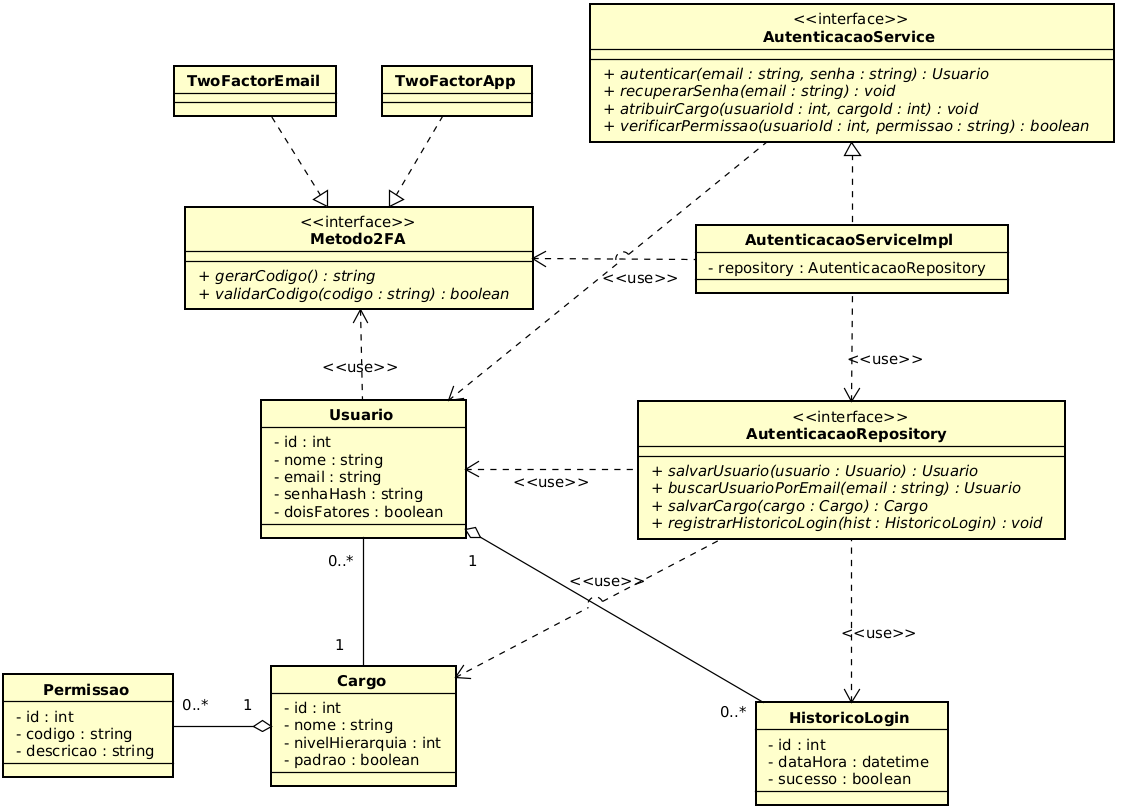
\includegraphics[width=\textwidth]{classes-autenticacao-acesso.png}
\caption{Diagrama de classes do componente de Autenticação e Acesso do EduHub. Fonte: elaboração própria da equipe.}
\label{fig:classes-autenticacao}
\end{figure}

O diagrama organiza as entidades
centrais do domínio de acesso, como \texttt{Usuario}, \texttt{Cargo},
\texttt{Permissao} e \texttt{HistoricoLogin}, em que cada usuário é associado a
um único cargo e cada cargo agrupa as permissões que definem o que seus
usuários podem fazer no sistema (RF-06, RF-10). A autenticação de dois fatores
(RNF-04) é modelada pela interface \texttt{Metodo2FA}, com as operações
\texttt{gerarCodigo()} e \texttt{validarCodigo()}, implementada pelas classes
concretas \texttt{TwoFactorEmail} e \texttt{TwoFactorApp}, o que permite
acrescentar novos meios de verificação sem alterar o restante do componente.
As regras de negócio são expostas pela interface \texttt{AutenticacaoService},
implementada por \texttt{AutenticacaoServiceImpl}, com operações como
\texttt{autenticar()}, \texttt{recuperarSenha()}, \texttt{atribuirCargo()} e
\texttt{verificarPermissao()}. A persistência é isolada pela interface
\texttt{Autenticacao\allowbreak Repository}, responsável por operações como
\texttt{salvarUsuario()}, \texttt{buscarUsuarioPorEmail()},
\texttt{salvarCargo()} e \texttt{registrarHistoricoLogin()}. Assim como no
Registro Acadêmico, essa separação entre serviço e repositório mantém as
regras de negócio independentes da tecnologia de persistência, em linha com o
objetivo de manutenibilidade (RNF-07).

\textbf{Registro Acadêmico:} Este componente concentra as
regras de negócio do processo de avaliação e controle de presença, com
forte dependência do conceito de período letivo travado/destravado
(RF-26, premissa P-4):
\begin{itemize}[nosep]
    \item o professor tem acesso exclusivo à lista de alunos e à estrutura
    de notas apenas das turmas e disciplinas às quais está vinculado
    (RF-21).
    \item o professor pode inserir notas parciais e finais por disciplina e
    por período letivo (RF-22) e editá-las (RF-23), desde que o período não
    tenha sido travado pela administração (RF-23, RF-26).
    \item o professor registra presença, falta ou justificativa de ausência
    por aluno, data e aula/período (RF-24).
    \item o sistema calcula automaticamente o total de faltas e o
    percentual de frequência por disciplina (RF-25).
    \item o usuário administrativo pode travar o lançamento de notas e
    frequência por período letivo a qualquer momento, impedindo qualquer
    alteração posterior pelos professores (RF-26). Conforme CU-03, se houver
    turmas ou disciplinas do período com notas finais ou frequência
    pendentes, o sistema apenas sinaliza essas pendências ao administrativo,
    sem impedir o travamento. Uma correção após o período travado exige que
    o professor solicite o destravamento à administração, que reabre o
    período pela função ``Desbloquear Período'', permite a correção e trava
    o período novamente.
    \item o professor pode visualizar, a partir da lista de chamada, os
    dados de contato do aluno cadastrados pelo administrativo (RF-27).
\end{itemize}

O projeto de classes correspondente ao componente de Registro Acadêmico é
apresentado na Figura~\ref{fig:classes-registro}.

\begin{figure}[ht]
\centering
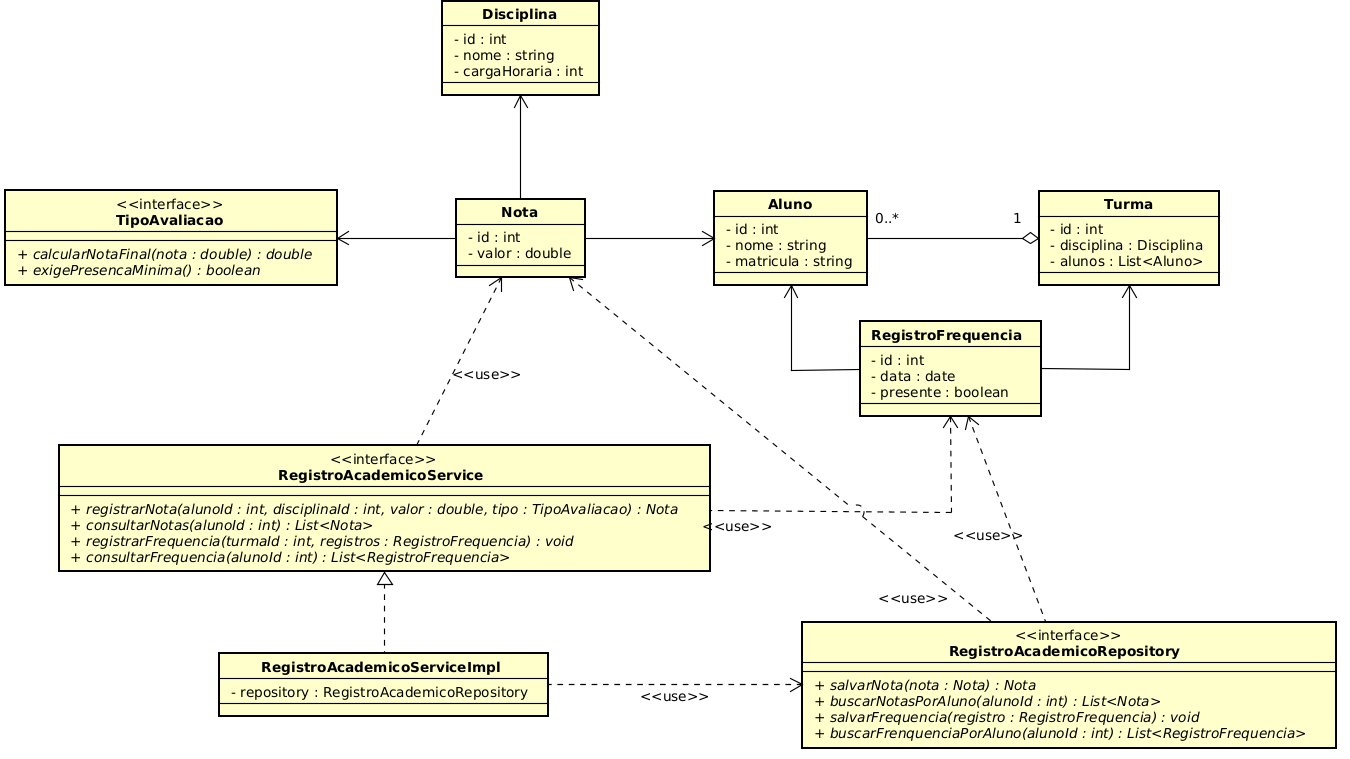
\includegraphics[width=\textwidth]{classes-registro-academico.png}
\caption{Diagrama de classes do componente de Registro Acadêmico do EduHub. Fonte: elaboração própria da equipe.}
\label{fig:classes-registro}
\end{figure}

O diagrama organiza as entidades centrais
do domínio acadêmico, como \texttt{Nota}, \texttt{Aluno}, \texttt{Turma},
\texttt{Disciplina} e \texttt{RegistroFrequencia}, e define a interface
\texttt{TipoAvaliacao}, com as operações \texttt{calcularNotaFinal()} e
\texttt{exigePresencaMinima()}, que abstrai os diferentes tipos de avaliação.
As regras de negócio são expostas pela interface
\texttt{RegistroAcademicoService}, implementada por
\texttt{RegistroAcademicoServiceImpl}, com operações como
\texttt{registrarNota()}, \texttt{consultarNotas()},
\texttt{registrarFrequencia()} e \texttt{consultarFrequencia()}. A
persistência é isolada pela interface \texttt{RegistroAcademicoRepository},
responsável por operações como \texttt{salvarNota()},
\texttt{buscarNotasPorAluno()}, \texttt{salvarFrequencia()} e
\texttt{buscarFrequenciaPorAluno()}. Essa separação entre serviço e
repositório mantém as regras de negócio independentes da tecnologia de
persistência, em linha com o objetivo de manutenibilidade (RNF-07).

O projeto de classes dos demais componentes será elaborado nas próximas
iterações, conforme cada um for detalhado.

\section{Princípios de projeto}

A equipe já tratava coesão e acoplamento como atributos de qualidade de
produto desde a etapa de especificação de requisitos, entendendo que, do
ponto de vista do desenvolvedor, a qualidade é medida pela implementação de
um código limpo, com alta coesão e baixo acoplamento, e associando esses
atributos diretamente à manutenibilidade (RNF-07). Já naquela etapa ficou
definido que a equipe monitoraria essas propriedades por meio de métricas
estáticas de produto, como o CBO (\emph{Coupling Between Object Classes}) e o
LCOM (\emph{Lack of Cohesion in Methods}), buscando manter CBO baixo e LCOM
próximo de zero.

Aplicado ao projeto de componentes do EduHub, esse princípio se traduz em
manter a separação de responsabilidades já estabelecida na divisão modular
do Capítulo 2: o componente de Controle de Acesso não deve conhecer as
regras de negócio de Gestão Acadêmica (por exemplo, cálculo de faltas ou
travamento de período letivo), e vice-versa. A relação entre eles deve se
limitar à consulta de permissão, verificando se o professor está autorizado a
lançar notas na turma. Da mesma forma, o componente de Relatórios e Auditoria
deve depender dos demais módulos apenas para leitura de dados, sem que módulos
como Gestão Acadêmica ou Cadastros precisem conhecer a lógica de geração de
relatórios. Essa baixa dependência mútua entre componentes é o que permite,
conforme RNF-07, adicionar novos recursos a um módulo sem impactar os
demais.

Além da coesão e do acoplamento, o projeto de classes do componente de
Autenticação e Acesso (Figura~\ref{fig:classes-autenticacao}) aplica três
princípios SOLID:
\begin{itemize}[nosep]
    \item \textbf{Responsabilidade Única (SRP)}: as entidades
    (\texttt{Usuario}, \texttt{Cargo}, \texttt{Permissao} e
    \texttt{HistoricoLogin}) representam apenas os dados e o estado, a interface
    \texttt{AutenticacaoService} concentra as regras de autenticação e de
    controle de acesso e a interface \texttt{Autenticacao\allowbreak Repository}
    cuida apenas da persistência.
    \item \textbf{Aberto/Fechado (OCP)}: a interface \texttt{Metodo2FA} deixa a
    autenticação de dois fatores aberta para extensão e fechada para
    modificação. Novos meios de verificação, como \texttt{TwoFactorEmail} e
    \texttt{TwoFactorApp}, são adicionados como classes concretas, e um
    eventual método por SMS entraria da mesma maneira, sem alterar o código
    existente.
    \item \textbf{Inversão de Dependência (DIP)}: a implementação
    \texttt{AutenticacaoServiceImpl} depende da abstração
    \texttt{Autenticacao\allowbreak Repository}, e não de uma tecnologia de
    persistência concreta, o que mantém as regras de controle de acesso
    independentes da infraestrutura.
\end{itemize}
Da mesma forma, o projeto de classes do componente de Registro Acadêmico
(Figura~\ref{fig:classes-registro}) aplica os mesmos três princípios:
\begin{itemize}[nosep]
    \item \textbf{Responsabilidade Única (SRP)}: cada classe tem um papel bem
    definido. As entidades (\texttt{Nota}, \texttt{Aluno}) representam apenas
    os dados e o estado, o serviço (\texttt{RegistroAcademicoService})
    concentra as regras de negócio e o repositório
    (\texttt{RegistroAcademicoRepository}) cuida apenas da persistência, o que
    facilita a manutenção e os testes isolados.
    \item \textbf{Aberto/Fechado (OCP)}: a interface \texttt{TipoAvaliacao}
    deixa o sistema aberto para extensão e fechado para modificação. Novos
    tipos de avaliação, como \texttt{AvaliacaoProva} e
    \texttt{AvaliacaoTrabalho}, são adicionados como classes concretas, sem
    alterar o código existente e sem recorrer a enumerações e a múltiplos
    condicionais.
    \item \textbf{Inversão de Dependência (DIP)}: a implementação
    \texttt{RegistroAcademicoServiceImpl} depende de abstrações, e não de
    detalhes técnicos. O \texttt{RegistroAcademicoRepository} oculta a
    tecnologia de persistência concreta, como MySQL, MongoDB ou uma API, o que
    mantém as regras de negócio independentes da infraestrutura.
\end{itemize}
Os princípios SOLID restantes, a Substituição de Liskov (LSP) e a Segregação
de Interface (ISP), e sua aplicação aos demais componentes serão detalhados
nas próximas iterações, conforme o projeto de classes de cada um for
elaborado.

\section{Padrões de projeto}

O projeto de classes apresentado na Seção~\ref{sec:detalhamento} e a divisão
em componentes do Capítulo 2 evidenciam padrões de projeto que se encaixam naturalmente nos problemas de
projeto do EduHub. Esta seção documenta os quatro padrões de encaixe mais
direto, indicando o problema que cada um resolve e um trecho de código
ilustrativo.

\textbf{Strategy (comportamental):} O componente de Registro Acadêmico
precisa calcular a nota final de diferentes tipos de avaliação, e o de
Autenticação e Acesso precisa validar diferentes métodos de segundo fator.
Tratar essas variações com uma cadeia de condicionais dentro do serviço
tornaria o código fechado à inclusão de novos tipos. O padrão Strategy
encapsula cada variação atrás de uma interface comum, deixando o serviço
independente da implementação concreta e permitindo acrescentar novos tipos
sem alterar o código existente, em conformidade com o princípio Aberto/Fechado.
Esse padrão já aparece no projeto de classes da Seção~\ref{sec:detalhamento},
nas interfaces \texttt{TipoAvaliacao} e \texttt{Metodo2FA}.

\begin{lstlisting}
interface TipoAvaliacao {
    double calcularNotaFinal(double nota);
    boolean exigePresencaMinima();
}
class AvaliacaoProva    implements TipoAvaliacao { /* ... */ }
class AvaliacaoTrabalho implements TipoAvaliacao { /* ... */ }

// o servico recebe a estrategia e nao conhece a implementacao concreta
double notaFinal = tipoAvaliacao.calcularNotaFinal(valor);
\end{lstlisting}

\textbf{Adapter (estrutural):} O EduHub envia notificações por meio de um
serviço de e-mail externo, cuja interface difere da esperada pelos componentes
internos. Como esse serviço é de terceiros e não pode ser modificado, o padrão
Adapter cria uma classe intermediária que implementa a interface interna
\texttt{Notificador} e traduz suas chamadas para a API externa. É esse o papel
do componente Adaptador de E-mail (RF-36).

\begin{lstlisting}
interface Notificador {
    void notificar(Usuario destino, String assunto, String corpo);
}

class AdaptadorEmail implements Notificador {
    private final ServicoEmailExterno externo; // API de terceiros, imutavel

    AdaptadorEmail(ServicoEmailExterno externo) { this.externo = externo; }

    public void notificar(Usuario destino, String assunto, String corpo) {
        // traduz a chamada interna para a API externa
        externo.send("no-reply@eduhub", destino.getEmail(), assunto, corpo);
    }
}
\end{lstlisting}

\textbf{Observer (comportamental):} Eventos como a publicação de um comunicado
(RF-35) ou o lançamento de uma nota exigem que vários destinos sejam
atualizados, como a caixa de entrada do aluno (RF-37) e o disparo de e-mail
(RF-36). Acoplar o produtor do evento a cada destino dificultaria a inclusão de
novos canais. O padrão Observer define uma relação um-para-muitos em que o
objeto observado notifica automaticamente todos os observadores registrados
quando seu estado muda.

\begin{lstlisting}
class EventoAcademico extends Subject {
    void publicarComunicado(Comunicado c) {
        this.comunicado = c;
        notifyObservers(); // avisa todos os canais registrados
    }
}
class CanalCaixaEntrada implements Observer {
    public void update(Subject s) { /* grava na caixa de entrada */ }
}
class CanalEmail implements Observer {
    public void update(Subject s) { /* dispara via AdaptadorEmail */ }
}
\end{lstlisting}

\textbf{Proxy de proteção (estrutural):} Regras como o acesso do professor
apenas às turmas às quais está vinculado (RF-21) e a restrição de alteração de
cargos a perfis administrativos (RF-07) exigem verificar a permissão antes de
executar a operação. Em vez de espalhar essa verificação pelas regras de
negócio, o padrão Proxy interpõe um objeto que implementa a mesma interface do
serviço real, verifica a permissão e apenas então delega a chamada.

\begin{lstlisting}
class RegistroAcademicoProxy implements RegistroAcademicoService {
    private final RegistroAcademicoService real;
    private final AutenticacaoService acesso;

    public Nota registrarNota(int alunoId, int disciplinaId,
                              double valor, TipoAvaliacao tipo) {
        if (!acesso.verificarPermissao(professorAtual(), "LANCAR_NOTA"))
            throw new AcessoNegado();
        return real.registrarNota(alunoId, disciplinaId, valor, tipo);
    }
}
\end{lstlisting}

\chapter{Projeto de Interface do Usuário}

Na etapa de Engenharia de Software I, a própria equipe produziu a
especificação de requisitos do EduHub, definindo restrições, requisitos
funcionais e não funcionais e histórias de usuário, mas sem chegar a
desenhar \textit{mockups} de interface. Este
capítulo parte desse trabalho anterior: primeiro deriva os princípios de
interface e os fluxos de interação mais relevantes a partir das restrições
e histórias já levantadas e, em seguida, apresenta os protótipos de alta
fidelidade produzidos no Figma para o fluxo mais crítico do sistema, o
caso de uso CU-03.

\section{Princípios de interface}

A interface do EduHub deve seguir os seguintes princípios, todos rastreáveis a
restrições e requisitos não funcionais do documento de requisitos:

\begin{itemize}
    \item \textbf{Aplicação web responsiva} (R-1): o sistema é acessado
    exclusivamente pelo navegador, sem aplicativo móvel nativo nesta versão.
    A interface deve, portanto, se adaptar a diferentes tamanhos de tela,
    especialmente para o perfil Aluno, para o qual a equipe previu maior
    uso em dispositivos móveis ao definir os perfis de usuário na etapa de
    requisitos.
    \item \textbf{Acessibilidade} (R-2 e RNF-10): a interface deve aderir às
    diretrizes WCAG 2.1, nível AA, garantindo o uso do sistema por pessoas com
    deficiência.
    \item \textbf{Intuitividade adaptada ao perfil} (RNF-09): a navegação deve
    ser clara e adequada ao nível de proficiência de cada grupo de usuário.
    Ao definir os perfis de usuário na etapa de requisitos, a equipe
    caracterizou essa necessidade de forma distinta por perfil:
    \begin{itemize}
        \item o \textbf{Aluno} tem baixo nível de acesso, foco em
        visualização de informações e alta expectativa de acessibilidade em
        dispositivos móveis;
        \item o \textbf{Professor} tem nível médio de acesso, foco pedagógico
        e realiza inserção frequente de dados (frequência e notas), exigindo
        uma interface intuitiva que reduza o esforço em tarefas repetitivas;
        \item o \textbf{Administrativo} tem alto nível de acesso e
        conhecimento médio de sistemas de gestão, realizando tarefas de
        cadastro e manutenção de dados mais complexas.
    \end{itemize}
    \item \textbf{Compatibilidade de navegadores} (P-2): a interface deve
    funcionar corretamente em Google Chrome e derivados do Chromium, Mozilla
    Firefox e Safari (versões recentes), sendo esses os únicos navegadores
    contemplados pelo escopo de teste e suporte.
\end{itemize}

\section{Fluxos principais de usuário}

Os fluxos a seguir foram derivados das histórias de usuário e dos casos de
uso da especificação de requisitos. Cada um representa uma tarefa central
para o respectivo perfil, e não uma tela específica.

\subsection{Autenticação e recuperação de senha (HU-01)}

Qualquer usuário do sistema (Aluno, Professor ou Administrativo) precisa
autenticar-se por e-mail e senha antes de acessar suas funcionalidades. Caso
o usuário não recorde a senha, ele deve conseguir solicitar sua recuperação
por meio de um link ou código enviado ao e-mail cadastrado (RF-02). A tarefa
do usuário é, portanto, concluir o acesso ao sistema de forma rápida e
segura. O histórico de login (RF-05) é registrado de forma transparente ao
usuário, sem exigir ação adicional dele.

\subsection{Lançamento de notas e registro de frequência (HU-13 e HU-14)}

Esse é o fluxo central do perfil Professor, que precisa inserir dados com
frequência regular. A partir da lista de turmas e disciplinas vinculadas a
ele (RF-21), o professor deve conseguir lançar e editar notas parciais e
finais por aluno e período (RF-22, RF-23), além de registrar, por aula ou
por data, o status de frequência de cada aluno: presente, ausente ou
justificado (RF-24). O sistema calcula automaticamente o percentual de
frequência (RF-25), sem exigir cálculo manual do professor. Caso o período
letivo já esteja bloqueado pela Coordenação (RF-26), a interface deve
impedir a edição e comunicar claramente esse impedimento, conforme
detalhado no caso de uso CU-03 (Apêndice~\ref{apx:requisitos}). Correções
após o bloqueio dependem de solicitação do professor à Coordenação, que
desbloqueia o período antes de qualquer nova edição.

\subsection{Consulta ao boletim pelo aluno (HU-16)}

O aluno acessa seu boletim para visualizar notas parciais e finais de todas
as disciplinas, organizadas por período letivo (RF-28), e o detalhamento da
sua frequência, incluindo datas de falta e percentual acumulado de presença
(RF-29). Trata-se de um fluxo essencialmente de leitura, alinhado ao perfil
de baixo nível de acesso e foco em visualização definido pela equipe para o
Aluno, e que deve responder rapidamente (RNF-01).

\subsection{Cadastro de usuários e gestão de cargos (HU-03 e HU-04)}

O Administrativo cadastra novos usuários preenchendo os campos obrigatórios
exigidos pelo sistema (RF-13), associando obrigatoriamente um cargo a cada
novo cadastro (RF-06). O mesmo perfil pode alterar dados de terceiros
(RF-11) e inativar usuários mediante confirmação (RF-12). De forma
complementar, o Administrativo pode criar cargos personalizados, definir sua
hierarquia (RF-08) e configurar as permissões associadas a cada cargo
(RF-10), sem poder excluir os cargos padrão do sistema (RF-09). Esse fluxo é
o mais complexo do sistema do ponto de vista de interface, compatível com o
maior nível de acesso e conhecimento médio de sistemas de gestão que a
equipe atribuiu ao perfil Administrativo ao definir os perfis de usuário.

\section{Protótipos de tela}

Para manter o escopo desta iteração enxuto, a prototipação no Figma
concentra-se no fluxo do caso de uso CU-03 (Finalizar e Bloquear Período de
Lançamento), o mais crítico do sistema por proteger a integridade do registro
acadêmico e por girar em torno da regra de trava de lançamento (RF-26). A
Tabela~\ref{tab:telas-figma} lista as telas desse fluxo, do lançamento de notas
e frequência pelo professor até o travamento do período pela coordenação,
associando cada uma ao perfil de usuário correspondente e aos requisitos que a
originam. Cada tela foi prototipada em alta fidelidade em duas versões, uma para
\textit{desktop} e outra para dispositivos móveis, evidenciando a
responsividade exigida pelo princípio R-1. As subseções a seguir apresentam uma
etapa do fluxo por vez, sempre com a versão \textit{desktop} à esquerda e a
versão mobile correspondente à direita, para comparação. Os protótipos dos
demais fluxos e casos de uso serão elaborados de forma incremental nas próximas
iterações.

\begin{table}[ht]
\centering
\caption{Telas do fluxo do CU-03 prototipadas no Figma.}\label{tab:telas-figma}
\begin{tabularx}{\textwidth}{p{0.06\textwidth} p{0.30\textwidth} p{0.16\textwidth} X}
\toprule
\textbf{ID} & \textbf{Tela} & \textbf{Perfil} & \textbf{Fluxo/requisitos relacionados} \\
\midrule
T-01 & Tela de login & Todos & Autenticação por e-mail e senha (HU-01, RF-01) \\
T-02 & Lançamento e edição de notas & Professor & Notas parciais e finais por turma e período, com edição bloqueada quando o período está travado (HU-13, RF-22, RF-23, RF-26) \\
T-03 & Registro de frequência (chamada) & Professor & Presença, falta ou justificativa por aula e cálculo automático de faltas (HU-14, RF-24, RF-25) \\
T-04 & Gestão e travamento de períodos letivos & Coordenação & Verificação de pendências, travamento do lançamento e registro em log de auditoria (CU-03, RF-26, RF-44) \\
\bottomrule
\end{tabularx}
\end{table}

\subsection{O fluxo do CU-03 escolhido}

O CU-03 (Finalizar e Bloquear Período de Lançamento) foi escolhido como fluxo a
prototipar por ser o ponto em que se encontram os dois perfis operacionais do
sistema, o Professor e a Coordenação, em torno da regra que garante a
integridade do registro acadêmico, a trava de lançamento por período (RF-26).
Ele exercita ao mesmo tempo a inserção frequente de dados do Professor (notas e
frequência) e a ação administrativa de encerramento do período, o que permite
demonstrar em um único fluxo tanto o estado editável quanto o estado bloqueado
das telas.

O fluxo, conforme detalhado no CU-03 do Apêndice~\ref{apx:requisitos}, percorre
as seguintes etapas:

\begin{enumerate}
    \item o usuário se autentica na tela de login (T-01), comum a todos os
    perfis;
    \item o Professor acessa suas turmas e, com o período letivo aberto,
    lança e edita as notas (T-02) e registra a frequência da turma (T-03);
    \item a Coordenação acompanha, na gestão de períodos letivos (T-04), o
    progresso de preenchimento de notas e frequência de todas as disciplinas do
    período;
    \item a Coordenação pode bloquear o período a qualquer momento: havendo
    disciplinas com notas ou frequência pendentes, o sistema apenas sinaliza
    essas pendências como aviso, sem impedir o bloqueio, e a Coordenação
    decide se bloqueia mesmo assim, o que altera o status do período para
    ``Bloqueado'' e registra a ação no log de auditoria (RF-44);
    \item a partir desse momento, a trava (RF-26) passa a valer, e o Professor
    que retornar à tela de lançamento encontra os campos desabilitados, sem
    conseguir alterar notas ou frequência do período encerrado;
    \item eventuais correções após o bloqueio dependem de solicitação do
    Professor à Coordenação, que reabre o período pela ação ``Desbloquear
    Período'', realiza os ajustes necessários e bloqueia o período novamente
    ao concluir.
\end{enumerate}

As telas cobrem propositalmente os dois estados do período, aberto e bloqueado,
justamente para tornar visível o efeito da trava, que é o cerne do caso de uso.

\subsection{Autenticação (T-01)}

O acesso ao sistema começa pela tela de login (Figura~\ref{fig:tela-login}),
comum a todos os perfis. O usuário informa e-mail e senha e dispõe do atalho
``Esqueci minha senha'' para a recuperação por e-mail (RF-02). A tela concretiza
a primeira etapa do CU-03 e a história de autenticação HU-01.

\comparativotela{images/tela-cu03-01-login.png}{images/tela-cu03-01-login-mobile.png}%
{T-01 -- Tela de login (desktop à esquerda, mobile à direita), comum a todos os perfis.}{fig:tela-login}

\subsection{Lançamento e edição de notas (T-02)}

Autenticado como Professor, o usuário chega à tela inicial
(Figura~\ref{fig:prof-home}), que lista suas turmas do período corrente, com o
progresso de lançamento de cada uma e atalhos diretos para ``Notas'' e
``Frequência''.

\comparativotela{images/tela-cu03-02-prof-home.png}{images/tela-cu03-02-prof-home-mobile.png}%
{Tela inicial do Professor (desktop à esquerda, mobile à direita), com as turmas do período e atalhos para notas e frequência.}{fig:prof-home}

Na tela de lançamento de notas com o período aberto
(Figura~\ref{fig:notas-aberto}), o Professor edita as notas parciais e finais de
cada aluno por avaliação (RF-22, RF-23). O cabeçalho indica o estado ``Aberto''
do período, e o sistema calcula automaticamente a média a partir da fórmula de
cada aluno, exibida na própria linha. As ações ``Salvar Notas'' e ``Lançar
Notas'' ficam habilitadas.

\comparativotela{images/tela-cu03-03-notas-aberto.png}{images/tela-cu03-03-notas-aberto-mobile.png}%
{T-02 -- Lançamento de notas com o período aberto (desktop à esquerda, mobile à direita): campos e ações habilitados.}{fig:notas-aberto}

\subsection{Registro de frequência (T-03)}

Ainda com o período aberto, o Professor registra a frequência da turma
(Figura~\ref{fig:frequencia-aberto}), marcando cada aluno como presente (P),
ausente (A) ou justificado (J) por aula e data (RF-24). O sistema totaliza as
faltas e calcula automaticamente o percentual de frequência de cada aluno
(RF-25), sinalizando em vermelho quem está abaixo do mínimo, sem exigir cálculo
manual do Professor.

\comparativotela{images/tela-cu03-04-frequencia-aberto.png}{images/tela-cu03-04-frequencia-aberto-mobile.png}%
{T-03 -- Registro de frequência (desktop à esquerda, mobile à direita) com cálculo automático do percentual (RF-25).}{fig:frequencia-aberto}

\subsection{Gestão e travamento de períodos letivos (T-04)}

Autenticada como Coordenação, a usuária chega à tela inicial
(Figura~\ref{fig:coord-home}), que lista os períodos letivos e seu estado
(aberto, com pendências ou fechado), com acesso aos detalhes de cada um.

\comparativotela{images/tela-cu03-05-coord-home.png}{images/tela-cu03-05-coord-home-mobile.png}%
{Tela inicial da Coordenação (desktop à esquerda, mobile à direita), com os períodos letivos e seus estados.}{fig:coord-home}

Ao abrir os detalhes do período (Figura~\ref{fig:periodo-aberto}), a Coordenação
vê, disciplina a disciplina, o progresso de lançamento de notas e frequência,
com o percentual de conclusão de cada uma. Esse painel corresponde à verificação
de pendências prevista no CU-03: o botão ``Bloquear Período'' fica sempre
disponível, e eventuais pendências de notas ou frequência aparecem apenas como
aviso, cabendo à Coordenação decidir se bloqueia o período mesmo assim.

\comparativotela{images/tela-cu03-06-periodo-aberto.png}{images/tela-cu03-06-periodo-aberto-mobile.png}%
{T-04 -- Gestão do período aberto (desktop à esquerda, mobile à direita): progresso por disciplina e ação de bloqueio (RF-26).}{fig:periodo-aberto}

Após o bloqueio, o status do período passa a ``Bloqueado''
(Figura~\ref{fig:periodo-bloqueado}), a ação de bloqueio é registrada no log de
auditoria (RF-44) e a opção disponível passa a ser ``Desbloquear Período'',
executada pela Coordenação quando o Professor solicita correções em notas ou
frequência já encerradas.

\comparativotela{images/tela-cu03-07-periodo-bloqueado.png}{images/tela-cu03-07-periodo-bloqueado-mobile.png}%
{T-04 -- Período após o bloqueio (desktop à esquerda, mobile à direita): status ``Bloqueado'' e opção de desbloqueio.}{fig:periodo-bloqueado}

\subsection{Efeito da trava sobre o Professor}

Fechado o círculo do CU-03, o Professor que retornar à tela de lançamento do
período agora bloqueado (Figura~\ref{fig:notas-bloqueado}) encontra os campos de
nota desabilitados e as ações de salvar e lançar inativas. O cabeçalho informa a
data em que o período foi fechado, comunicando claramente o impedimento previsto
no RF-26. Essa tela é a contraparte da Figura~\ref{fig:notas-aberto} e torna
visível, na interface, o resultado da trava aplicada pela Coordenação.

\comparativotela{images/tela-cu03-08-notas-bloqueado.png}{images/tela-cu03-08-notas-bloqueado-mobile.png}%
{T-02 no estado bloqueado (desktop à esquerda, mobile à direita): campos e ações desabilitados pela trava de lançamento (RF-26).}{fig:notas-bloqueado}

\chapter{Especificação e Estratégia de Testes}

\section{Planejamento e níveis de teste}

A estratégia de testes do EduHub contempla três níveis, cada um com um
objetivo específico dentro do contexto do sistema:

\begin{itemize}
    \item \textbf{Testes de unidade}: verificam isoladamente regras de
    negócio críticas do domínio acadêmico, como o cálculo automático de
    frequência (RF-25), a trava de lançamento por período (RF-26) e a
    prevenção de conflitos de horário (RF-19). Como essas regras envolvem
    lógica de decisão relativamente isolada, o teste de unidade é o nível
    mais eficiente para capturar defeitos nelas o quanto antes.
    \item \textbf{Testes de integração}: verificam a comunicação entre os
    módulos do sistema, por exemplo, entre o módulo de autenticação e o de
    gestão de cargos/permissões, ou entre o módulo de cadastros (turmas,
    disciplinas, professores) e o módulo acadêmico (notas, frequência), que
    depende diretamente dos vínculos criados no cadastro.
    \item \textbf{Testes de sistema}: verificam o comportamento fim a fim das
    histórias de usuário, sob a perspectiva do usuário final, cobrindo os
    critérios de aceitação já descritos em cada história (por exemplo, o
    login em menos de dois segundos, previsto no critério de aceitação da
    HU-01 e no RNF-01).
\end{itemize}

Requisitos considerados críticos para a priorização dos testes são a
autenticação (RF-01, RF-02, RNF-03), o cálculo automático de frequência
(RF-25), a trava de lançamento de notas e frequência (RF-26) e a prevenção
de conflitos de horário (RF-19), por afetarem diretamente a integridade dos
dados acadêmicos e o controle de acesso ao sistema.

\section{Testes de unidade}

As unidades a seguir foram selecionadas por representarem regras de negócio
com lógica de decisão bem delimitada, derivadas diretamente dos requisitos
funcionais:

\begin{table}[ht]
\centering
\caption{Cenários de teste de unidade derivados dos requisitos funcionais.}
\begin{tabularx}{\textwidth}{p{0.16\textwidth} X X}
\toprule
\textbf{Unidade (RF)} & \textbf{Entrada/condição} & \textbf{Resultado esperado} \\
\midrule
Cálculo de percentual de frequência (RF-25) &
Total de aulas registradas e número de faltas de um aluno em uma disciplina &
Percentual de frequência calculado corretamente e exibido sem intervenção manual \\
Validação de conflito de horário (RF-19) &
Tentativa de atribuir um professor ou uma turma a um horário/sala já ocupado por outro professor ou turma &
O sistema rejeita a atribuição e sinaliza o conflito, sem alterar os dados existentes \\
Trava de lançamento por período (RF-26) &
Tentativa de edição de nota ou frequência em um período marcado como ``travado'' &
A edição é bloqueada e uma mensagem informa que o período está encerrado \\
Validação de campos obrigatórios (RF-13) &
Cadastro de novo usuário com um ou mais campos obrigatórios não preenchidos &
O sistema impede o salvamento e indica os campos pendentes \\
\bottomrule
\end{tabularx}
\end{table}

Para unidades que dependem de recursos externos ao próprio módulo, como o
envio de e-mail de recuperação de senha (RF-02) ou de notificações (RF-36),
a equipe pretende utilizar substitutos controlados (\textit{stubs} ou
\textit{mocks}) para isolar a lógica testada do envio real, evitando que a
disponibilidade de serviços externos interfira no resultado do teste.

\section{Testes de integração}

Os módulos do EduHub, autenticação/autorização, cadastros (usuários,
turmas, disciplinas, professores), acadêmico (notas e frequência) e
comunicação (avisos e mensagens), possuem dependências diretas entre si: o
módulo acadêmico depende dos vínculos criados no módulo de cadastros
(RF-17), e todos os módulos dependem da autenticação e das permissões de
cargo (RF-06, RF-10) para autorizar cada ação.

A estratégia adotada é a integração incremental do tipo \textit{bottom-up}:
os módulos de autenticação e de cadastros, por serem a base sobre a qual os
demais módulos operam, são testados primeiro, o que também é coerente com
a ordem que a equipe definiu no planejamento das sprints: a Primeira
Iteração cobre autenticação e cadastro de usuários, e a Segunda Iteração
cobre turmas, disciplinas e alocação de professores. Somente após essa base
estar validada os módulos acadêmico e de comunicação, que dependem dela, são
integrados e testados.

A cada alteração relevante em um módulo já integrado, testes de regressão
são reexecutados sobre os módulos que dependem dele, de forma a identificar
rapidamente efeitos colaterais não previstos. Por exemplo, uma alteração
na regra de permissões de cargo deve reexecutar os testes de integração dos
módulos de cadastros e acadêmico, que dependem dela para autorizar ações.

\section{Critérios de conclusão e cobertura}

Uma funcionalidade é considerada testada de forma satisfatória quando todos
os cenários de teste planejados para os RFs/RNFs associados à respectiva
história de usuário foram executados, o critério de aceitação descrito na
história de usuário correspondente (Apêndice~\ref{apx:requisitos}) foi
verificado, e não há defeito conhecido que bloqueie o critério final da
sprint em que a história está inserida.

A cobertura de código é utilizada como um indicador complementar do esforço
de teste, e não como garantia isolada de qualidade. Um código totalmente
coberto ainda pode conter regras de negócio mal validadas. Como meta
inicial proposta pela equipe, busca-se cobrir prioritariamente as unidades
críticas listadas na Seção 5.2. Essa meta poderá ser revisada ao longo do
projeto.

Além da cobertura, a estratégia de testes se relaciona com as métricas de
produto e de uso que a equipe definiu na etapa de requisitos. Do lado do
produto, o acompanhamento do acoplamento entre classes (CBO), da coesão dos
métodos (LCOM) e da complexidade ciclomática ajuda a identificar trechos de
código mais difíceis de testar e manter. Do lado do uso, a taxa de sucesso,
o tempo de conclusão de tarefas e o questionário SUS (\textit{System
Usability Scale}) complementam os testes automatizados ao avaliar a
experiência real do usuário nos fluxos descritos no Capítulo 4.

\section{Automação e ferramentas}

A execução dos testes de unidade e de integração e a
geração de relatórios de resultado são automatizadas pela esteira de
integração contínua do projeto, o GitHub Actions
(Seção~\ref{sec:build-cicd}), acionada a cada \textit{commit} e
\textit{pull request}, o que garante a reexecução frequente prevista na
estratégia de regressão descrita na Seção 5.3. Para as métricas de produto
definidas pela equipe (CBO, LCOM e complexidade ciclomática), a mesma
esteira executa uma etapa de análise estática de código. As ferramentas específicas
de execução de testes e de análise estática dependem da linguagem e do
\textit{framework} escolhidos para a implementação e são integradas ao GitHub
Actions por meio de scripts de \textit{build} e teste versionados junto ao
código.

\chapter{Gestão de Configuração e Manutenção}

\section{Repositório e itens de configuração}\label{sec:config-repo}

A gestão do Scrumban adotado pela equipe é feita no Taiga, utilizado para
o rastreamento do product backlog e das sprints, e o código-fonte é
versionado no GitHub, que funciona como repositório central do projeto, com o
Git como sistema de controle de versão.

O versionamento no GitHub segue um modelo de branches inspirado no Git Flow,
com dois branches de longa duração: a \texttt{main}, que reflete o código em
produção, e a \texttt{develop}, que reúne o trabalho já integrado e serve de
base para o ambiente de homologação. Cada nova funcionalidade ou correção é
desenvolvida em um branch próprio de curta duração (\texttt{feature/*}),
criado a partir da \texttt{develop}, e retorna a ela por meio de um
\textit{pull request} (PR) revisado. Quando o conteúdo da \texttt{develop}
está estável e validado, ele é promovido para a \texttt{main}, caracterizando
uma nova entrega em produção.

Os seguintes itens de configuração precisam ser controlados ao longo do
projeto:

\begin{itemize}
    \item código-fonte do sistema;
    \item documentação do projeto, incluindo o documento de requisitos (ES1)
    e este documento de projeto (ES2);
    \item modelos e diagramas (diagrama de classes e diagramas de caso de
    uso);
    \item testes (de unidade, integração e sistema, conforme o Capítulo 5);
    \item arquivos de configuração do sistema;
    \item o product backlog e as histórias de usuário, mantidos no Taiga.
\end{itemize}

\section{Gestão de dependências e alterações}

O projeto possui uma dependência externa relevante (D-1): a alocação e
configuração de um servidor de produção pela equipe de TI da instituição de
ensino. Como essa dependência está fora do controle direto da equipe de
desenvolvimento, ela é acompanhada como um risco de cronograma para a fase
de implantação, e não como um item versionado pela equipe.

Para as alterações internas ao sistema, a arquitetura modular exigida pelo
RNF-07, que prevê que novos recursos possam ser adicionados sem impactar
negativamente os módulos existentes, limita o alcance de cada alteração a
um módulo (ou a poucos módulos relacionados), reduzindo o risco de efeitos
colaterais quando uma história de usuário é implementada.

A coerência entre código, testes e documentação é mantida pelo próprio
processo Scrumban adotado pela equipe: o product backlog é um artefato
vivo, refinado continuamente, de modo que qualquer
alteração de escopo em uma história de usuário é refletida no backlog antes
de ser implementada, evitando divergência entre o que está documentado e o
que é efetivamente desenvolvido e testado.

\section{Rastreabilidade}

A rastreabilidade no EduHub segue a cadeia definida na própria estrutura da
especificação de requisitos (Apêndice~\ref{apx:requisitos}): requisitos
funcionais/não funcionais (RFs/RNFs) são agrupados em histórias de usuário,
cada uma listando explicitamente os ``RFs/RNFs associados'', e as histórias
de usuário são alocadas pela equipe às sprints do product backlog. A tabela a seguir
ilustra essa cadeia com dois exemplos concretos:

\begin{table}[ht]
\centering
\caption{Exemplos de rastreabilidade entre requisitos, histórias de usuário e sprints.}
\begin{tabularx}{\textwidth}{p{0.24\textwidth} X p{0.14\textwidth}}
\toprule
\textbf{Requisitos (RFs/RNFs)} & \textbf{História(s) de usuário} & \textbf{Sprint} \\
\midrule
RF-01, RF-02, RF-05 & HU-01 (Autenticação e Segurança) & 1\textsuperscript{a} Iteração \\
RF-15, RF-17 & HU-08 (Criação de Turmas e Disciplinas), HU-09 (Alocação de Professores) & 2\textsuperscript{a} Iteração \\
\bottomrule
\end{tabularx}
\end{table}

\section{\textit{Build}, integração e entrega}\label{sec:build-cicd}

O processo de entrega do EduHub seguirá o modelo Scrumban adotado
pelo projeto: entregas incrementais ao final de cada sprint de 14 dias, cada
uma correspondendo a um incremento funcional do produto, conforme o critério
final que a equipe define para cada sprint no planejamento. Por exemplo, a Primeira
Iteração tem como critério final permitir login e o cadastro de ao menos um
usuário professor. A automação de \textit{build}, integração contínua e
entrega (CI/CD) é realizada no GitHub, por meio do GitHub Actions, apoiada no
modelo de branches descrito na Seção~\ref{sec:config-repo}. A integração
contínua (CI) é acionada a cada \textit{commit} e a cada \textit{pull request},
executando o \textit{build} do sistema, os testes automatizados de unidade e
integração descritos no Capítulo 5 e a análise estática de código. Um
\textit{pull request} só é incorporado à \texttt{develop} quando essa
verificação passa, o que impede que código defeituoso avance. A entrega
contínua (CD) é acionada nas integrações aos branches de ambiente: ao chegar à
\texttt{develop}, a versão é publicada automaticamente no ambiente de
homologação, usado para validação antes da produção, e, ao ser promovida para
a \texttt{main}, é implantada no ambiente de produção.

\chapter*{Controle de Versões do Documento}
\addcontentsline{toc}{chapter}{Controle de Versões do Documento}

Esta seção registra o histórico de alterações significativas deste
documento de projeto. O versionamento do software em si é tratado no
Capítulo 6, na Seção de \textit{Build}, integração e entrega.

\begin{table}[ht]
\centering
\caption{Histórico de versões do documento.}
\begin{tabularx}{0.95\textwidth}{p{0.21\textwidth} p{0.19\textwidth} p{0.12\textwidth} X}
\toprule
\textbf{Data} & \textbf{Autor(es)} & \textbf{Versão} & \textbf{Alteração} \\
\midrule
25/08/2026 & Equipe EduHub & 1.0 & Versão inicial da documentação de projeto (ES2), consolidada a partir do documento de requisitos (ES1). \\
\bottomrule
\end{tabularx}
\end{table}


% ============================================================================
% APÊNDICES
% ============================================================================
\appendix
\chapter{Especificação Detalhada de Requisitos}\label{apx:requisitos}

Este apêndice apresenta a especificação completa de requisitos do EduHub,
elaborada pela própria equipe no Documento de Especificação de Requisitos de
Software (SRS) do projeto: os 45 requisitos funcionais, os 10 requisitos não
funcionais, as 18 histórias de usuário e os 3 casos de uso que representam o
escopo inicial do sistema.

\section{Requisitos Funcionais}

\subsection{Acesso e Autenticação}

\begin{xltabular}{\textwidth}{p{0.10\textwidth} p{0.20\textwidth} p{0.14\textwidth} X}
\caption{Requisitos funcionais -- Acesso e Autenticação.}\label{tab:rf-acesso}\\
\toprule
\textbf{ID} & \textbf{Requisito} & \textbf{Prioridade} & \textbf{Descrição} \\
\midrule
\endfirsthead
\toprule
\textbf{ID} & \textbf{Requisito} & \textbf{Prioridade} & \textbf{Descrição} \\
\midrule
\endhead
\bottomrule
\endlastfoot
RF-01 & Autenticação por Credencial & Alta & O sistema deve apresentar uma interface de login onde qualquer usuário pode se autenticar utilizando seu e-mail e uma senha. \\
RF-02 & Recuperação de Senha & Média & O sistema deve permitir que o usuário solicite a recuperação de senha através do envio de um link ou código de redefinição para o seu e-mail cadastrado. \\
RF-03 & Visualização de Perfil Próprio & Baixa & Qualquer usuário autenticado deve ser capaz de acessar e visualizar seus próprios dados cadastrais e de contato. \\
RF-04 & Alteração de Dados Pessoais & Média & O usuário deve ser capaz de alterar dados de seu perfil pessoal, exceto o e-mail. \\
RF-05 & Registro de Histórico de Login & Baixa & O sistema deve registrar o histórico de login de todos os usuários, incluindo data, hora e o endereço IP de acesso, para fins de segurança e auditoria. \\
RF-06 & Associação de Cargo & Alta & No momento da criação, todo novo usuário deve ser obrigatoriamente associado a um cargo específico que define suas permissões e hierarquia. \\
RF-07 & Designação de Cargo & Alta & O usuário com permissão administrativa deve ser capaz de designar (ou alterar) o cargo de qualquer outro usuário do sistema. \\
RF-08 & Criação e Hierarquia de Cargos & Alta & O cliente (Administrativo) deve ser capaz de criar novos cargos personalizados e definir o nível de hierarquia associado a cada um. \\
RF-09 & Cargos Padrões do Sistema & Média & O sistema deve conter cargos padrões que não podem ser excluídos, mas que podem ter seus nomes de exibição alterados pelo cliente. \\
RF-10 & Definição de Permissões Específicas & Alta & O cliente (administrativo) deve ser capaz de definir permissões específicas para cada cargo criado ou padrão. \\
RF-11 & Alteração de Dados de Terceiros & Média & O usuário com permissão administrativa deve ser capaz de alterar os dados cadastrais e de perfil de qualquer outro usuário do sistema. \\
RF-12 & Exclusão/Inativação de Usuários & Baixa & O usuário com permissão administrativa deve ser capaz de excluir (ou inativar) usuários do sistema, exigindo uma confirmação da ação antes da exclusão permanente. \\
RF-13 & Preenchimento Obrigatório & Alta & O sistema deve exigir o preenchimento de campos obrigatórios para o cadastro de qualquer novo usuário. \\
\end{xltabular}

\subsection{Gestão e Estrutura}

\begin{table}[H]
\centering
\caption{Requisitos funcionais -- Gestão e Estrutura.}
\begin{tabularx}{\textwidth}{p{0.10\textwidth} p{0.20\textwidth} p{0.14\textwidth} X}
\toprule
\textbf{ID} & \textbf{Requisito} & \textbf{Prioridade} & \textbf{Descrição} \\
\midrule
RF-14 & Gestão de Dados da Escola & Alta & O usuário administrativo deve ser capaz de cadastrar e atualizar os dados da escola no sistema, incluindo nome, endereço e informações de contato. \\
RF-15 & Criação de Turmas e Disciplinas & Média & O usuário administrativo deve ser capaz de criar, editar e desativar registros de turmas e disciplinas. \\
RF-16 & Configuração de Horários & Baixa & O usuário administrativo deve ser capaz de configurar os horários de funcionamento da escola (turnos e dias letivos) e definir o calendário acadêmico com eventos, feriados e datas importantes. \\
RF-17 & Vínculo Professor-Disciplina & Média & O usuário administrativo deve ser capaz de vincular professores a turmas e disciplinas específicas, definindo quais matérias o docente está autorizado a lecionar. \\
RF-18 & Busca Avançada de Cadastros & Baixa & O sistema deve permitir ao administrativo a busca por alunos, professores, turmas, disciplinas e salas utilizando filtros como nome, ID/matrícula, ano/semestre ou cargo. \\
RF-19 & Restrição de Conflito de Horário & Baixa & O sistema deve impedir a atribuição de dois professores ou duas turmas diferentes ao mesmo horário e mesma sala de aula, exibindo uma mensagem de erro em caso de conflito. \\
RF-20 & Gestão de Períodos de Matrícula & Baixa & O cliente (administrativo) deve ser capaz de abrir e encerrar períodos de matrícula e de revalidação de matrícula no sistema. \\
\bottomrule
\end{tabularx}
\end{table}

\subsection{Gestão Acadêmica}

\begin{table}[H]
\centering
\caption{Requisitos funcionais -- Gestão Acadêmica.}
\begin{tabularx}{\textwidth}{p{0.10\textwidth} p{0.20\textwidth} p{0.14\textwidth} X}
\toprule
\textbf{ID} & \textbf{Requisito} & \textbf{Prioridade} & \textbf{Descrição} \\
\midrule
RF-21 & Acesso à Disciplina e Turma & Baixa & O professor deve ter acesso exclusivo para visualizar a lista de alunos e a estrutura de notas apenas para as turmas e disciplinas às quais está vinculado. \\
RF-22 & Lançamento de Notas & Alta & O professor deve ser capaz de inserir as notas parciais e finais de cada aluno, por disciplina e por período letivo, através de uma interface clara. \\
RF-23 & Edição de Notas & Média & O professor deve ser capaz de editar notas inseridas, desde que o período de lançamento/edição não tenha sido travado pela administração. \\
RF-24 & Registro de Frequência & Alta & O professor deve ser capaz de registrar a presença (Frequente), falta (Ausente) ou justificativa de ausência de cada aluno, por data e por aula/período. \\
RF-25 & Cálculo Automático de Faltas & Alta & O sistema deve calcular e exibir automaticamente o total de faltas e o percentual de frequência do aluno em cada disciplina. \\
RF-26 & Trava de Lançamento & Baixa & O sistema deve permitir ao usuário administrativo travar o lançamento de notas e frequência por período letivo, impedindo qualquer alteração posterior pelos Professores. \\
RF-27 & Visualização de Detalhes do Aluno & Baixa & O professor deve ser capaz de visualizar, a partir da lista de chamada, os detalhes de contato (telefone, e-mail) do aluno, conforme cadastrado pelo administrativo. \\
\bottomrule
\end{tabularx}
\end{table}

\subsection{Informação e Consulta do Aluno}

\begin{table}[H]
\centering
\caption{Requisitos funcionais -- Informação e Consulta do Aluno.}
\begin{tabularx}{\textwidth}{p{0.10\textwidth} p{0.20\textwidth} p{0.14\textwidth} X}
\toprule
\textbf{ID} & \textbf{Requisito} & \textbf{Prioridade} & \textbf{Descrição} \\
\midrule
RF-28 & Consulta ao Boletim Individual & Alta & O aluno deve ser capaz de visualizar seu boletim completo, exibindo as notas parciais e finais de todas as disciplinas, organizado por período letivo. \\
RF-29 & Consulta Detalhada de Frequência & Baixa & O aluno deve ser capaz de visualizar o detalhe de sua frequência em cada disciplina, incluindo a data das faltas e o percentual acumulado de presença. \\
RF-30 & Visualização da Grade de Horários & Média & O aluno deve ser capaz de consultar sua grade de horários de aula semanal, exibindo a disciplina e o nome do professor para cada bloco de horário. \\
RF-31 & Informações do Professor & Baixa & Ao consultar uma disciplina, o aluno deve ser capaz de visualizar o nome completo e o e-mail institucional do professor responsável por aquela matéria. \\
RF-32 & Consulta ao Calendário Acadêmico & Média & O aluno deve ser capaz de visualizar o calendário acadêmico publicado pela administração, incluindo feriados, datas de provas e eventos importantes. \\
RF-33 & Solicitação de Documentos & Alta & O aluno deve ser capaz de iniciar e submeter uma solicitação formal por documentos através de um formulário no sistema. \\
RF-34 & Acompanhamento de Solicitações & Baixa & O aluno deve ser capaz de visualizar o status de suas solicitações de documentos. \\
\bottomrule
\end{tabularx}
\end{table}

\subsection{Comunicação e Notificações}

\begin{table}[H]
\centering
\caption{Requisitos funcionais -- Comunicação e Notificações.}
\begin{tabularx}{\textwidth}{p{0.10\textwidth} p{0.20\textwidth} p{0.14\textwidth} X}
\toprule
\textbf{ID} & \textbf{Requisito} & \textbf{Prioridade} & \textbf{Descrição} \\
\midrule
RF-35 & Envio de Comunicados (Admin) & Alta & O usuário administrativo deve ser capaz de criar, redigir e enviar comunicados ou avisos a grupos específicos de usuários. \\
RF-36 & Envio de Notificações por E-mail & Média & O sistema deve enviar notificações por e-mail para eventos importantes e configuráveis. \\
RF-37 & Caixa de Entrada do Aluno & Alta & O aluno deve ter uma caixa de entrada no sistema para receber e visualizar todos os comunicados e mensagens enviadas pela administração. \\
RF-38 & Criação de Mensagem do Aluno & Média & O aluno deve ser capaz de iniciar e enviar uma nova mensagem de consulta à administração através de um formulário. \\
RF-39 & Tags de Assunto Obrigatórias & Baixa & O sistema deve exigir que o aluno selecione uma tag de assunto predefinida ao enviar uma mensagem para a administração. \\
RF-40 & Roteamento de Mensagens por Tag & Baixa & O sistema deve rotear a mensagem do aluno, baseada na tag de assunto selecionada, para a equipe administrativa responsável. \\
RF-41 & Registro de Histórico de Mensagens & Baixa & O sistema deve manter o registro e o histórico de todas as mensagens trocadas entre alunos e a administração, acessível apenas por usuários administrativos com permissão. \\
\bottomrule
\end{tabularx}
\end{table}

\subsection{Relatórios e Auditoria}

\begin{table}[H]
\centering
\caption{Requisitos funcionais -- Relatórios e Auditoria.}
\begin{tabularx}{\textwidth}{p{0.10\textwidth} p{0.20\textwidth} p{0.14\textwidth} X}
\toprule
\textbf{ID} & \textbf{Requisito} & \textbf{Prioridade} & \textbf{Descrição} \\
\midrule
RF-42 & Geração de Relatórios Acadêmicos & Baixa & O sistema deve permitir ao administrativo gerar relatórios consolidados sobre frequência e desempenho dos alunos, com opções de filtro por turma, disciplina e período letivo. \\
RF-43 & Exportação de Relatórios & Baixa & Os relatórios gerados devem poder ser exportados no formato de arquivo PDF. \\
RF-44 & Log de Alterações & Baixa & O sistema deve manter um registro (log) de todas as alterações feitas em dados cadastrais críticos. \\
RF-45 & Consulta ao Log de Auditoria & Baixa & Apenas usuários com permissão de administrador devem ser capazes de consultar e filtrar o documento de log. \\
\bottomrule
\end{tabularx}
\end{table}

\section{Requisitos Não Funcionais}

\subsection{Desempenho}

\begin{table}[H]
\centering
\caption{Requisitos não funcionais -- Desempenho.}
\begin{tabularx}{\textwidth}{p{0.12\textwidth} p{0.24\textwidth} X}
\toprule
\textbf{ID} & \textbf{Requisito} & \textbf{Descrição} \\
\midrule
RNF-01 & Tempo de Resposta Crítica & O tempo de resposta para qualquer operação crítica deve ser inferior a 2 segundos em condições normais de uso. \\
RNF-02 & Capacidade de Transação & O sistema deve ser capaz de processar até 10.000 transações por minuto durante períodos de pico. \\
\bottomrule
\end{tabularx}
\end{table}

\subsection{Segurança}

\begin{table}[H]
\centering
\caption{Requisitos não funcionais -- Segurança.}
\begin{tabularx}{\textwidth}{p{0.12\textwidth} p{0.24\textwidth} X}
\toprule
\textbf{ID} & \textbf{Requisito} & \textbf{Descrição} \\
\midrule
RNF-03 & Criptografia de Dados Sensíveis & O sistema deve criptografar em repouso todos os dados cadastrais que envolvem documentos e informações pessoais (incluindo senhas e e-mails). \\
RNF-04 & Autenticação de Dois Fatores (2FA) & O sistema deve oferecer suporte opcional para autenticação de dois fatores (2FA) para os perfis de administrativo e docente. \\
\bottomrule
\end{tabularx}
\end{table}

\subsection{Confiabilidade e Disponibilidade}

\begin{table}[H]
\centering
\caption{Requisitos não funcionais -- Confiabilidade e Disponibilidade.}
\begin{tabularx}{\textwidth}{p{0.12\textwidth} p{0.24\textwidth} X}
\toprule
\textbf{ID} & \textbf{Requisito} & \textbf{Descrição} \\
\midrule
RNF-05 & Disponibilidade Mínima & O sistema deve ter uma disponibilidade mínima de 99\% por ano. \\
RNF-06 & Backups e Restauração & O sistema deve realizar backups automáticos diários de todos os dados e ser capaz de restaurar o sistema completamente a partir de um backup. \\
\bottomrule
\end{tabularx}
\end{table}

\subsection{Manutenibilidade e Portabilidade}

\begin{table}[H]
\centering
\caption{Requisitos não funcionais -- Manutenibilidade e Portabilidade.}
\begin{tabularx}{\textwidth}{p{0.12\textwidth} p{0.24\textwidth} X}
\toprule
\textbf{ID} & \textbf{Requisito} & \textbf{Descrição} \\
\midrule
RNF-07 & Arquitetura Modular & O sistema deve ser desenvolvido com uma arquitetura modular, permitindo que novos recursos e funcionalidades sejam adicionados sem impactar negativamente a operação dos módulos existentes. \\
RNF-08 & Suporte a Múltiplas Plataformas & O software deve funcionar corretamente em todas as plataformas mais utilizadas: Web (Chrome, Firefox, Safari), Windows e macOS; a solução deve ser uma aplicação web responsiva que funcione bem nesses ambientes. \\
\bottomrule
\end{tabularx}
\end{table}

\subsection{Usabilidade e Acessibilidade}

\begin{table}[H]
\centering
\caption{Requisitos não funcionais -- Usabilidade e Acessibilidade.}
\begin{tabularx}{\textwidth}{p{0.12\textwidth} p{0.24\textwidth} X}
\toprule
\textbf{ID} & \textbf{Requisito} & \textbf{Descrição} \\
\midrule
RNF-09 & Intuitividade da Interface & A interface do usuário deve ser intuitiva, com navegação clara e fácil, adaptada ao nível de proficiência e necessidades dos perfis de usuário (Aluno, Professor, Administrativo). \\
RNF-10 & Acessibilidade & O sistema deve ser acessível para pessoas com deficiência, atendendo às diretrizes WCAG 2.1. \\
\bottomrule
\end{tabularx}
\end{table}

\section{Histórias de Usuário}

As histórias de usuário a seguir representam os requisitos funcionais e não
funcionais sob a perspectiva do usuário, agrupadas conforme os módulos do
sistema. Elas representam o escopo inicial do projeto; outras histórias
serão definidas e implementadas de forma incremental conforme o
desenvolvimento progredir. A Tabela~\ref{tab:hu-resumo} apresenta um resumo
de todas as 18 histórias, seguida do detalhamento de cada uma (história e
critério de aceitação).

\begin{xltabular}{\textwidth}{p{0.07\textwidth} p{0.25\textwidth} p{0.14\textwidth} p{0.14\textwidth} X}
\caption{Resumo das histórias de usuário.}\label{tab:hu-resumo}\\
\toprule
\textbf{ID} & \textbf{Título} & \textbf{Prioridade} & \textbf{Estimativa} & \textbf{RFs/RNFs associados} \\
\midrule
\endfirsthead
\toprule
\textbf{ID} & \textbf{Título} & \textbf{Prioridade} & \textbf{Estimativa} & \textbf{RFs/RNFs associados} \\
\midrule
\endhead
\bottomrule
\endlastfoot
HU-01 & Autenticação e Segurança & Alta & 5 dias & RF-01, RF-02, RF-05, RNF-01, RNF-03, RNF-04 \\
HU-02 & Gestão de Dados Pessoais e Perfil & Média & 2 dias & RF-03, RF-04 \\
HU-03 & Criação e Manutenção de Usuários & Alta & 4 dias & RF-06, RF-11, RF-12, RF-13 \\
HU-04 & Criação e Gestão de Cargos & Alta & 3 dias & RF-08, RF-09, RF-10 \\
HU-05 & Atribuição de Cargo ao Usuário & Média & 1 dia & RF-07 \\
HU-06 & Gestão da Escola e Infraestrutura & Média & 1 dia & RF-14, RF-15 \\
HU-07 & Configuração do Período Acadêmico & Média & 2 dias & RF-16, RF-20 \\
HU-08 & Criação de Turmas e Disciplinas & Alta & 4 dias & RF-15 \\
HU-09 & Alocação de Professores & Alta & 4 dias & RF-17 \\
HU-10 & Prevenção de Conflitos de Agendamento & Média & 3 dias & RF-19 \\
HU-11 & Busca e Pesquisa de Cadastros & Alta & 2 dias & RF-18 \\
HU-12 & Visualização de Turmas e Acesso & Alta & 2 dias & RF-21, RNF-01 \\
HU-13 & Lançamento e Edição de Notas & Alta & 6 dias & RF-22, RF-23, RF-26, RNF-02 \\
HU-14 & Registro Diário de Frequência & Alta & 4 dias & RF-24, RF-25, RNF-02 \\
HU-15 & Consulta Rápida de Contato do Aluno & Alta & 1 dia & RF-27 \\
HU-16 & Consulta Detalhada do Desempenho & Média & 3 dias & RF-28, RF-29, RNF-01 \\
HU-17 & Visualização da Grade e Calendário & Média & 3 dias & RF-30, RF-31, RF-32 \\
HU-18 & Solicitação e Acompanhamento de Documentos & Média & 3 dias & RF-33, RF-34 \\
\end{xltabular}

\subsection{Histórias de Usuário sobre Acesso e Autenticação}

\paragraph{HU-01 -- Autenticação e Segurança.}
\textit{História:} Como um usuário, eu quero fazer login no sistema de forma
segura e rápida, e poder recuperar a senha se necessário, para que eu possa
acessar minhas informações em menos de um segundo.
\textit{Critério de Aceitação:} O usuário deve conseguir logar em menos de 2
segundos (RNF-01). O link de recuperação deve ser enviado. O histórico de
login deve ser registrado (RF-05).

\paragraph{HU-02 -- Gestão de Dados Pessoais e Perfil.}
\textit{História:} Como um usuário, eu quero acessar minha página de perfil
e atualizar minhas informações de contato e senha, para que meus dados
pessoais estejam sempre corretos e atualizados.
\textit{Critério de Aceitação:} O usuário deve visualizar todos os seus
dados (RF-03) e conseguir alterar campos editáveis (exceto e-mail) com
sucesso. A nova senha deve ser salva criptografada.

\paragraph{HU-03 -- Criação e Manutenção de Usuários.}
\textit{História:} Como um administrativo, eu quero cadastrar, alterar
dados de terceiros e inativar usuários (alunos e professores), para que eu
possa gerenciar o acesso à plataforma e manter o cadastro da escola
atualizado.
\textit{Critério de Aceitação:} O administrativo consegue cadastrar um novo
usuário (RF-13) e a associação a um cargo (RF-06) é obrigatória. O
administrativo deve conseguir alterar dados (RF-11) e excluir/inativar
(RF-12) qualquer usuário.

\paragraph{HU-04 -- Criação e Gestão de Cargos.}
\textit{História:} Como um administrativo, eu quero criar novos cargos
personalizados, hierarquizá-los e especificar quais permissões cada cargo
possui, para que eu possa atender às necessidades de segurança e funções
específicas da escola.
\textit{Critério de Aceitação:} O administrativo consegue criar um novo
cargo (RF-08) e customizar as permissões (RF-10). Cargos padrões (RF-09)
não podem ser excluídos.

\paragraph{HU-05 -- Atribuição de Cargo ao Usuário.}
\textit{História:} Como um administrativo, eu quero designar ou mudar o
cargo de um usuário existente, para que eu possa controlar o nível de
acesso dele ao sistema de acordo com sua função atual.
\textit{Critério de Aceitação:} O administrativo deve conseguir alterar o
cargo de um usuário (RF-07) e as permissões de acesso do usuário devem ser
atualizadas imediatamente com base no novo cargo.

\subsection{Histórias de Usuário sobre Gestão e Estrutura}

\paragraph{HU-06 -- Gestão da Escola e Infraestrutura.}
\textit{História:} Como um administrativo, eu quero cadastrar e atualizar
os dados da escola.
\textit{Critério de Aceitação:} O administrativo deve conseguir cadastrar
(RF-14) e editar os dados da escola.

\paragraph{HU-07 -- Configuração do Período Acadêmico.}
\textit{História:} Como um administrativo, eu quero definir os horários de
funcionamento, criar o calendário acadêmico e gerenciar os períodos de
matrícula, para que o ano letivo esteja formalmente estruturado.
\textit{Critério de Aceitação:} O administrativo deve conseguir configurar
os horários de turnos, cadastrar eventos no calendário (RF-16) e
abrir/encerrar períodos de matrícula (RF-20).

\paragraph{HU-08 -- Criação de Turmas e Disciplinas.}
\textit{História:} Como um administrativo, eu quero criar, editar e
desativar turmas e disciplinas, para que a estrutura curricular esteja
atualizada antes do início das aulas.
\textit{Critério de Aceitação:} O administrativo consegue criar, editar e
desativar turmas e disciplinas (RF-15).

\paragraph{HU-09 -- Alocação de Professores.}
\textit{História:} Como um administrativo, eu quero vincular um professor a
turmas e disciplinas específicas, para que ele tenha permissão para
lançar notas e frequência.
\textit{Critério de Aceitação:} O administrativo deve conseguir atribuir um
professor a uma ou mais disciplinas (RF-17).

\paragraph{HU-10 -- Prevenção de Conflitos de Agendamento.}
\textit{História:} Como um administrativo, eu quero ser alertado quando
houver conflitos de sala ou professor ao montar a grade de horários, para
que a grade de aulas seja logicamente válida.
\textit{Critério de Aceitação:} O sistema deve impedir (e exibir erro) a
atribuição de dois professores ou turmas diferentes ao mesmo horário e sala
(RF-19).

\paragraph{HU-11 -- Busca e Pesquisa de Cadastros.}
\textit{História:} Como um administrativo, eu quero buscar por qualquer
cadastro (aluno, professor, turma) usando vários filtros (nome, ID, ano),
para que eu possa encontrar informações rapidamente e gerenciar os dados.
\textit{Critério de Aceitação:} A busca deve retornar resultados filtrando
por nome, ID/matrícula, ano/semestre ou cargo (RF-18).

\subsection{Histórias de Usuário sobre Gestão Acadêmica}

\paragraph{HU-12 -- Visualização de Turmas e Acesso.}
\textit{História:} Como um professor, eu quero acessar rapidamente a lista
de turmas e disciplinas que leciono, para que eu possa iniciar o
lançamento de dados acadêmicos (notas e frequência).
\textit{Critério de Aceitação:} O professor deve ver apenas as turmas e
disciplinas vinculadas a ele (RF-21). O acesso deve ser rápido (RNF-01).

\paragraph{HU-13 -- Lançamento e Edição de Notas.}
\textit{História:} Como um professor, eu quero inserir e editar as notas
parciais e finais dos alunos em minhas disciplinas, para que o boletim do
aluno seja atualizado com precisão.
\textit{Critério de Aceitação:} O professor deve conseguir inserir e editar
todas as notas (RF-22, RF-23). A edição deve ser bloqueada se o período
estiver travado (RF-26).

\paragraph{HU-14 -- Registro Diário de Frequência.}
\textit{História:} Como um professor, eu quero registrar a presença, falta
ou justificativa de ausência dos alunos em minhas aulas, para que o
controle de frequência esteja correto e em dia.
\textit{Critério de Aceitação:} O professor deve conseguir registrar o
status de frequência por aluno e data (RF-24). O sistema deve calcular
automaticamente as faltas e percentuais (RF-25).

\paragraph{HU-15 -- Consulta Rápida de Contato do Aluno.}
\textit{História:} Como um professor, eu quero visualizar os dados de
contato dos alunos que leciono, para que eu possa comunicar urgências ou
dúvidas pontuais.
\textit{Critério de Aceitação:} O sistema deve exibir os detalhes de
contato (telefone, e-mail) do aluno e responsável na interface de gestão
(RF-27).

\subsection{Histórias de Usuário sobre Informação e Consulta do Aluno}

\paragraph{HU-16 -- Consulta Detalhada do Desempenho.}
\textit{História:} Como um aluno, eu quero acessar meu boletim com notas e
o detalhe da minha frequência em cada disciplina, para que eu possa
monitorar meu desempenho e presença.
\textit{Critério de Aceitação:} O aluno deve visualizar notas (RF-28) e o
percentual de faltas e datas (RF-29). O tempo de consulta deve ser rápido
(RNF-01).

\paragraph{HU-17 -- Visualização da Grade e Calendário.}
\textit{História:} Como um aluno, eu quero consultar minha grade de
horários, o calendário acadêmico e as informações do meu professor, para
que eu possa me organizar para as aulas e eventos.
\textit{Critério de Aceitação:} O aluno deve conseguir visualizar a grade
de horários completa (RF-30) e o calendário (RF-32), incluindo informações
de contato do professor (RF-31).

\paragraph{HU-18 -- Solicitação e Acompanhamento de Documentos.}
\textit{História:} Como aluno, eu quero solicitar documentos formais (ex:
histórico escolar) pelo sistema e acompanhar o status dessa solicitação,
para que eu não precise ir pessoalmente à Secretaria.
\textit{Critério de Aceitação:} O aluno deve conseguir submeter um
formulário de solicitação (RF-33) e verificar se o status está ``Em
Análise'', ``Aprovado'' ou ``Atendido'' (RF-34).

\section{Casos de Uso}

Os casos de uso a seguir fornecem uma descrição narrativa detalhada das
interações entre os atores (usuário, professor e administrativo) e o
sistema, com foco nas funcionalidades críticas ou mais complexas do
sistema. Representam o foco inicial do projeto, sendo que outros serão
refinados e implementados de forma incremental conforme o desenvolvimento
progredir. Os casos de uso CU-01 e CU-02 contam com diagramas de caso de uso
UML elaborados na fase de modelagem (Figuras~\ref{fig:cu01} e~\ref{fig:cu02});
para o CU-03 não foi produzido diagrama próprio nessa fase, sendo descrito
apenas de forma textual.

\subsection*{CU-01 -- Designar Cargo de Usuário}

\begin{tabularx}{\textwidth}{p{0.22\textwidth} X}
\toprule
\textbf{Ator Primário} & Usuário Administrativo \\
\textbf{Ator Secundário} & Usuário comum (Professor, Aluno, etc.) \\
\textbf{Pré-condições} & O administrador está logado no sistema. O usuário-alvo está cadastrado e existe no sistema. \\
\bottomrule
\end{tabularx}

\textbf{Fluxo Principal:}
\begin{enumerate}[nosep]
    \item O Administrador acessa a funcionalidade de Gestão de Usuários.
    \item O Administrador busca e seleciona o usuário desejado.
    \item O Sistema exibe os detalhes do usuário.
    \item O Administrador seleciona o novo Cargo/Função (ex: Professor, Coordenador) a ser atribuído.
    \item O Sistema valida o Cargo/Função.
    \item O Sistema atualiza o perfil do usuário (RF-07).
    \item O Sistema registra a alteração no Log de Auditoria (RF-44) e exibe uma mensagem de confirmação.
\end{enumerate}

\textbf{Fluxos Alternativos:}
\begin{itemize}[nosep]
    \item \textit{2.a.1.} O Sistema informa que o usuário buscado não foi encontrado (RF-18).
    \item \textit{4.a.1.} O Administrador tenta atribuir um cargo que não existe ou que é logicamente inválido.
    \item \textit{4.a.2.} O Sistema rejeita a ação e exibe uma mensagem de erro.
\end{itemize}

\textbf{Pós-condições:} O usuário-alvo tem o novo cargo/função designado. As
permissões de acesso do usuário são imediatamente atualizadas conforme o
novo cargo (RF-10).

\begin{figure}[ht]
\centering
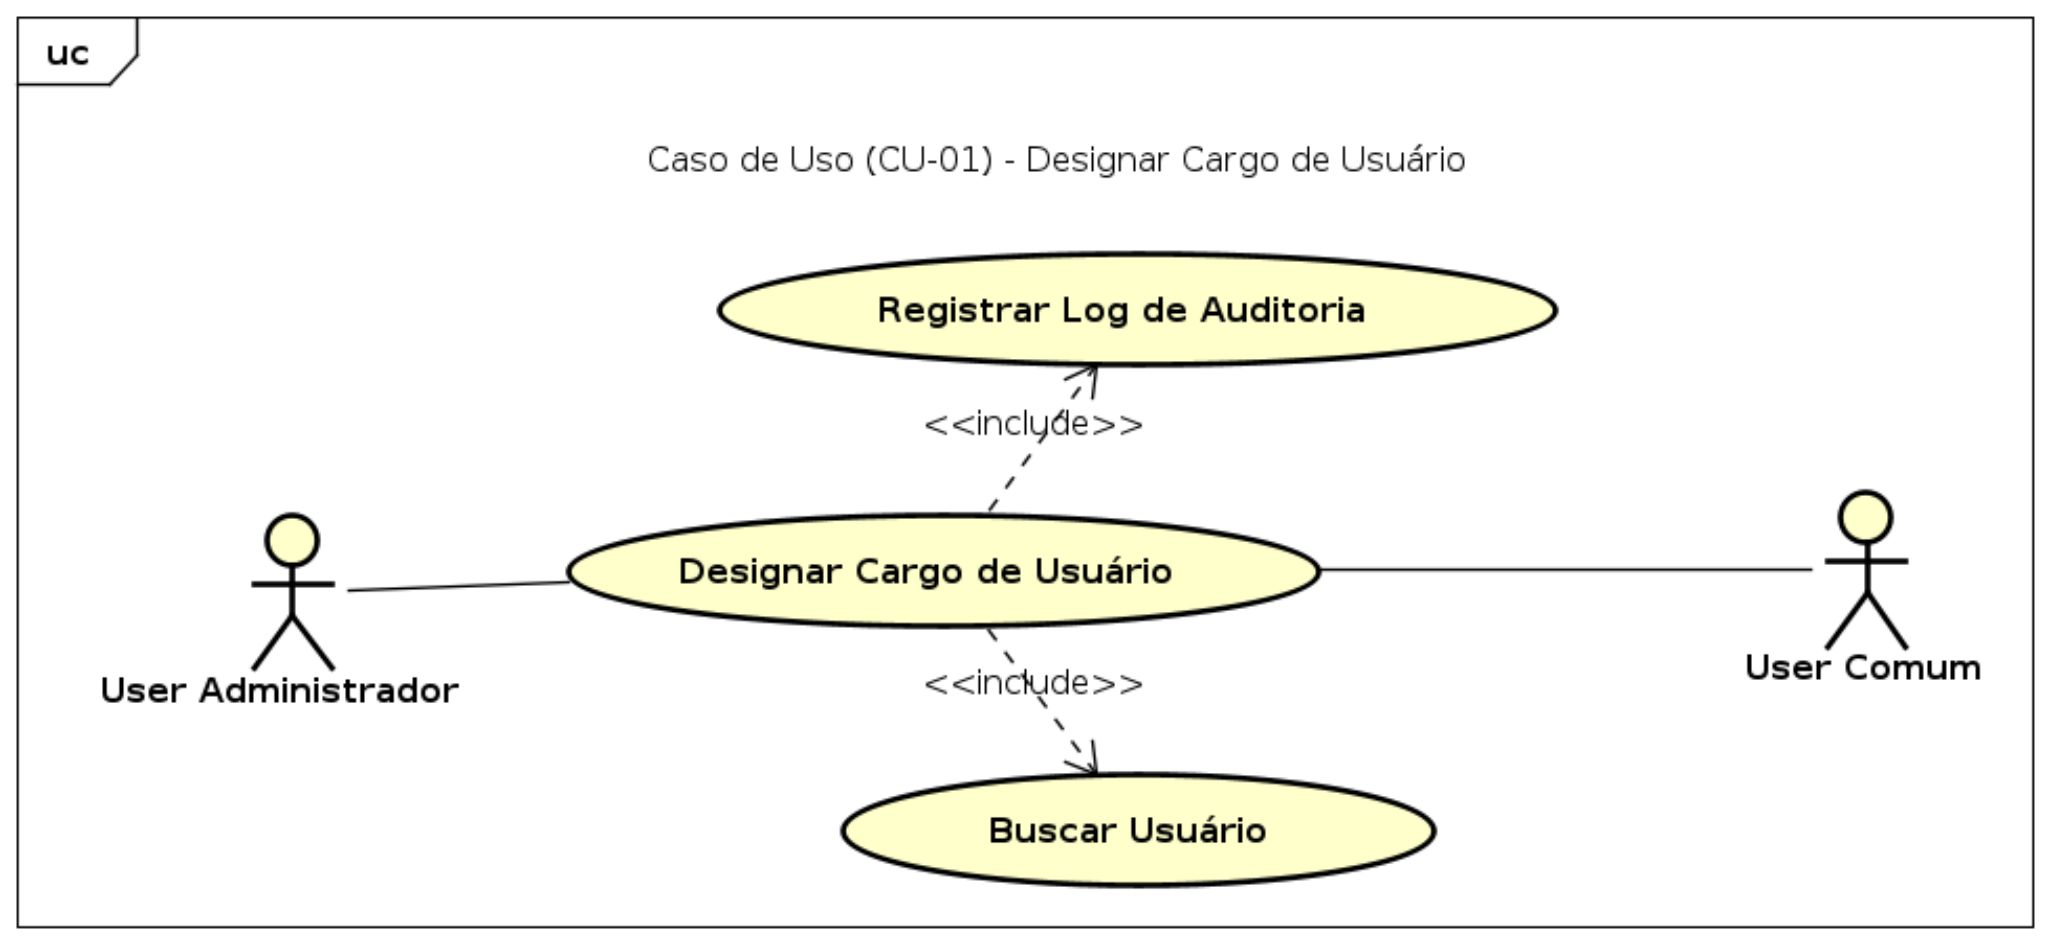
\includegraphics[width=0.9\textwidth]{diagrama-cu01.png}
\caption{Diagrama de caso de uso CU-01 -- Designar Cargo de Usuário. Fonte:
elaboração própria da equipe.}
\label{fig:cu01}
\end{figure}

\subsection*{CU-02 -- Alocar Professor/Turma e Prevenir Conflito}

\begin{tabularx}{\textwidth}{p{0.22\textwidth} X}
\toprule
\textbf{Ator Primário} & Usuário Administrativo \\
\textbf{Ator Secundário} & Usuário Professor \\
\textbf{Pré-condições} & O Administrativo está autenticado e a Sala, Turma e Professor já estão cadastrados. \\
\bottomrule
\end{tabularx}

\textbf{Fluxo Principal:}
\begin{enumerate}[nosep]
    \item O Administrativo acessa a tela de Configuração de Horários.
    \item O Administrativo seleciona a Turma, a Disciplina, o Professor, a Sala e o Horário (dia/período).
    \item O Sistema verifica se a Sala está disponível naquele horário para a Turma (RF-19).
    \item O Sistema verifica se o Professor está disponível naquele horário (RF-19).
    \item As verificações são aprovadas e o Administrativo salva o vínculo (RF-17).
\end{enumerate}

\textbf{Fluxos Alternativos:}
\begin{itemize}[nosep]
    \item \textit{3.a.1.} O Sistema detecta que a Sala já está ocupada por outra Turma ou Professor no mesmo horário.
    \item \textit{3.a.2.} O Sistema exibe uma mensagem de erro e lista o agendamento conflitante.
    \item \textit{4.a.1.} O Sistema detecta que o Professor já está alocado em outra Turma/Sala no mesmo horário.
    \item \textit{4.a.2.} O Sistema exibe uma mensagem de erro indicando o conflito na agenda do Docente.
\end{itemize}

\textbf{Pós-condições:} O vínculo Professor-Turma-Disciplina-Sala foi
criado e a agenda do sistema foi atualizada com sucesso, ou o sistema
impediu o agendamento e manteve os dados inalterados.

\begin{figure}[ht]
\centering
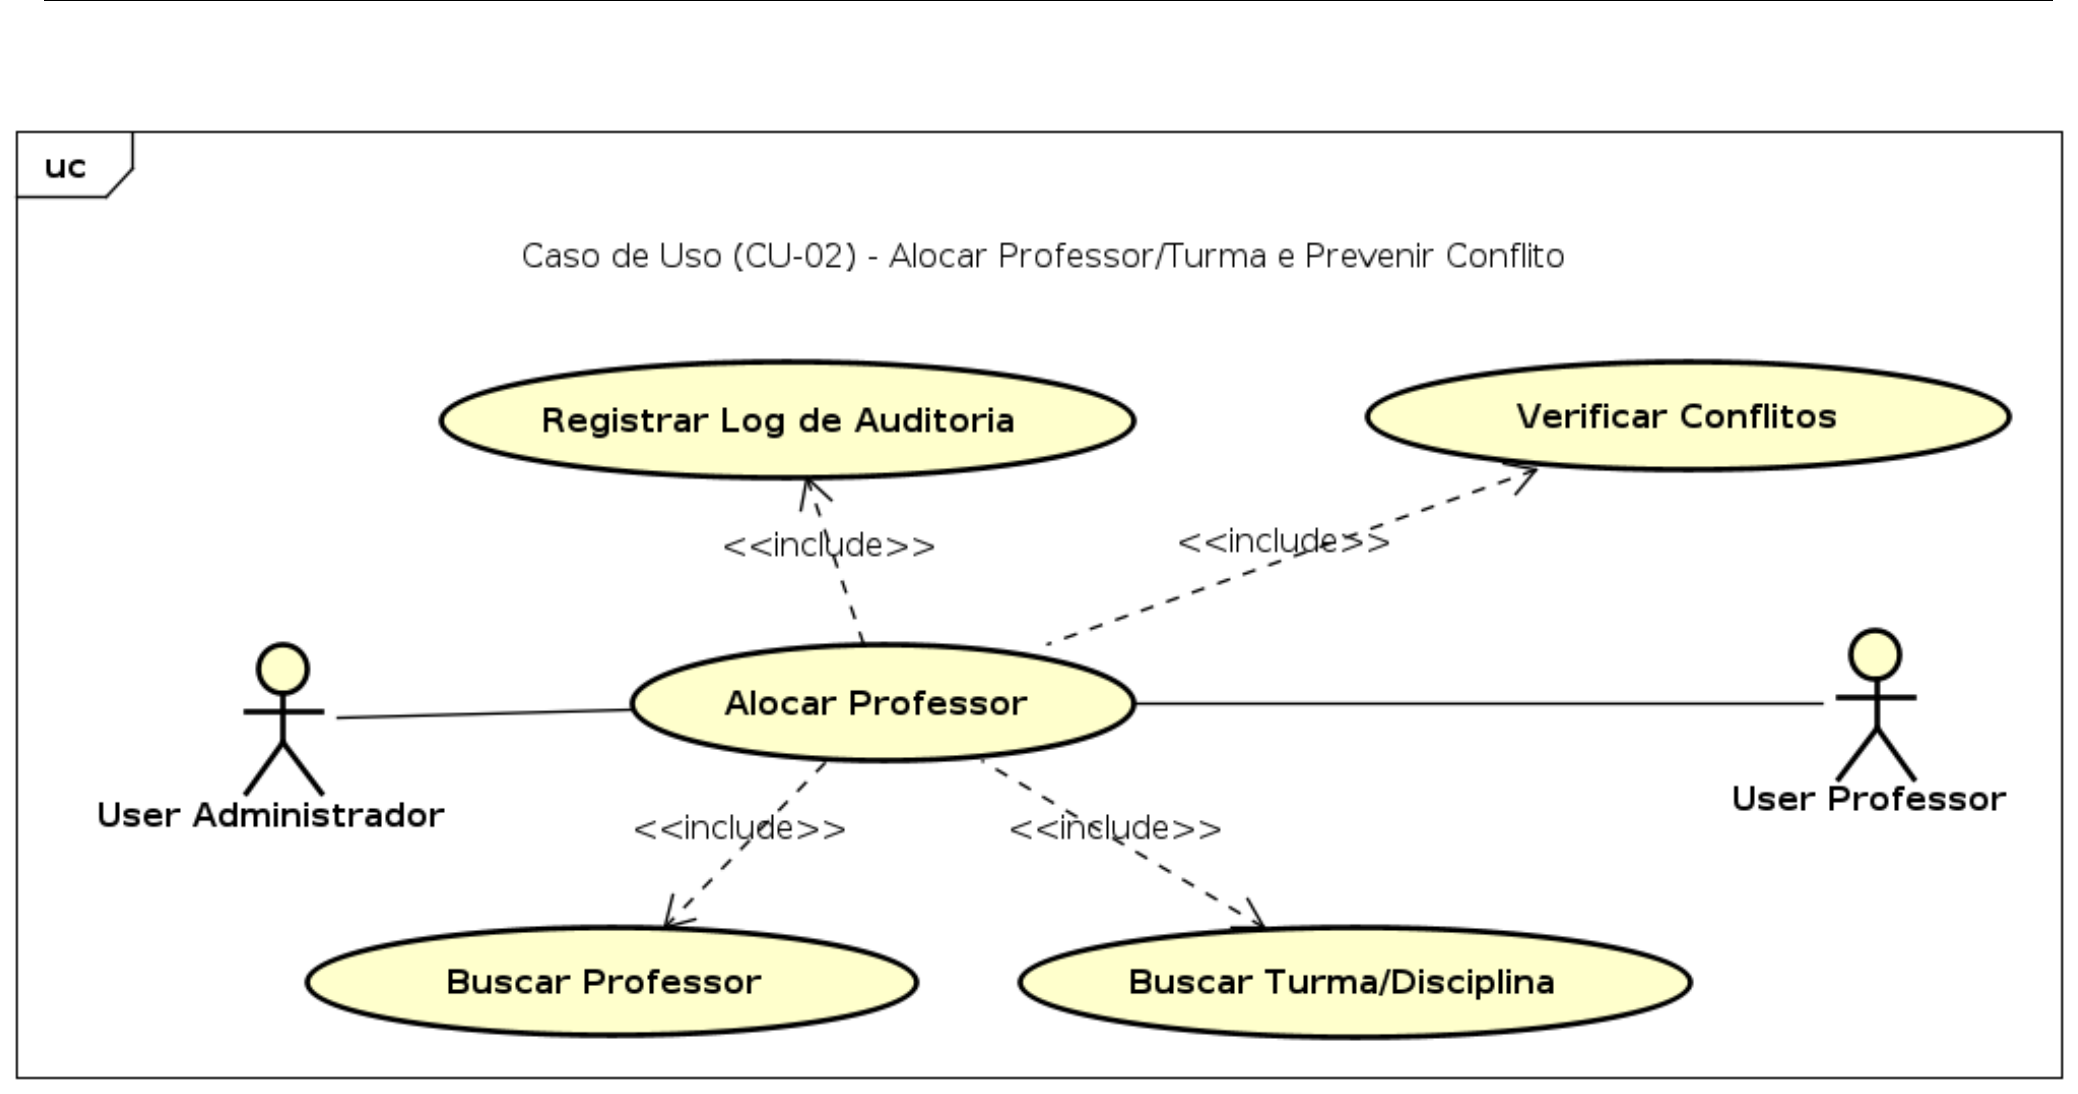
\includegraphics[width=0.9\textwidth]{diagrama-cu02.png}
\caption{Diagrama de caso de uso CU-02 -- Alocar Professor/Turma e Prevenir
Conflito. Fonte: elaboração própria da equipe.}
\label{fig:cu02}
\end{figure}

\subsection*{CU-03 -- Finalizar e Bloquear Período de Lançamento}

\begin{tabularx}{\textwidth}{p{0.22\textwidth} X}
\toprule
\textbf{Ator Primário} & Usuário Administrativo (ou Coordenador) \\
\textbf{Ator Secundário} & Usuário Professor \\
\textbf{Pré-condições} & O Administrador está autenticado. O Período Letivo a ser bloqueado existe e está com status ``Aberto''. \\
\bottomrule
\end{tabularx}

\textbf{Fluxo Principal:}
\begin{enumerate}[nosep]
    \item O Administrador/Coordenador acessa a funcionalidade de Gestão de Períodos Letivos.
    \item O Administrador seleciona o Período Letivo (ex: 1º Semestre de 2026) e escolhe a opção ``Travar Lançamento'' (RF-26).
    \item O Sistema verifica se há Turmas ou Disciplinas com notas finais ou frequência pendentes e, caso existam, exibe essas pendências como um aviso informativo (ex: ``4 Notas Finais e 2 Lançamentos de Frequência pendentes na disciplina de Matemática 3ºA''), sem impedir a continuação do fluxo.
    \item O Administrador/Coordenador confirma o bloqueio do Período, mesmo havendo pendências sinalizadas.
    \item O Sistema altera o status do Período para ``Bloqueado''.
    \item O Sistema registra o evento no Log de Auditoria (RF-44), incluindo quem fez a ação e a data/hora.
    \item O Sistema exibe uma mensagem de sucesso.
\end{enumerate}

\textbf{Fluxos Alternativos:}
\begin{itemize}[nosep]
    \item \textit{5.a.1.} Um Professor tenta acessar a tela de Lançamento de Notas para um Período com status ``Bloqueado''.
    \item \textit{5.a.2.} O Sistema verifica o status ``Bloqueado'' e exibe uma mensagem: ``Período encerrado para lançamentos. Consulte a Coordenação'' (RF-26).
    \item \textit{7.a.1.} Após o bloqueio, o Professor identifica que ainda precisa lançar ou corrigir uma nota ou frequência.
    \item \textit{7.a.2.} O Professor solicita à Coordenação o desbloqueio do Período.
    \item \textit{7.a.3.} A Coordenação acessa a Gestão de Períodos Letivos e seleciona a opção ``Desbloquear Período''.
    \item \textit{7.a.4.} O Sistema altera o status do Período de volta para ``Aberto'' e registra o evento no Log de Auditoria (RF-44).
    \item \textit{7.a.5.} O Professor realiza a correção ou o lançamento pendente.
    \item \textit{7.a.6.} A Coordenação bloqueia o Período novamente, repetindo o Fluxo Principal.
\end{itemize}

\textbf{Pós-condições:} O status do Período Acadêmico está definido como
``Bloqueado'' na Base de Dados. Qualquer tentativa de alteração de notas ou
frequência para este período é negada (RF-26). O Log de Auditoria (RF-44)
registra a ação de bloqueio. O Período pode ser reaberto pela Coordenação a
qualquer momento, mediante solicitação do Professor, através da
funcionalidade de Desbloquear Período.


% ============================================================================
% REFERÊNCIAS
% ============================================================================
% Sem referências bibliográficas nesta versão (documento derivado do próprio SRS/ES1).

\end{document}
